\documentclass[oldfontcommands,oneside,a4paper,11pt]{article} 
\RequirePackage{lineno} 
\usepackage{xunicode}%packages de base pour utiliser xetex
\usepackage{fontspec}
\usepackage{natbib}
\usepackage{booktabs}
\usepackage{xltxtra} 
\usepackage{longtable}
\usepackage{tangutex2} 
\usepackage{tangutex4} 
\usepackage{polyglossia} 
\usepackage[table]{xcolor}
\usepackage{gb4e} 
\usepackage{multicol}
\usepackage{graphicx}
\usepackage{float}
\usepackage{hyperref} 
\hypersetup{bookmarks=false,bookmarksnumbered,bookmarksopenlevel=5,bookmarksdepth=5,xetex,colorlinks=true,linkcolor=blue,citecolor=blue}
\usepackage[all]{hypcap}
\usepackage{memhfixc}
\usepackage{lscape}
\bibpunct[: ]{(}{)}{,}{a}{}{,}
%%%%%%%%%quelques options de style%%%%%%%%
%\setsecheadstyle{\SingleSpacing\LARGE\scshape\raggedright\MakeLowercase}
%\setsubsecheadstyle{\SingleSpacing\Large\itshape\raggedright}
%\setsubsubsecheadstyle{\SingleSpacing\itshape\raggedright}
%\chapterstyle{veelo}
%\setsecnumdepth{subsubsection}
%%%%%%%%%%%%%%%%%%%%%%%%%%%%%%%
\setmainfont[Mapping=tex-text,Numbers=OldStyle,Ligatures=Common]{Charis SIL} %ici on définit la police par défaut du texte
\renewcommand \thesection {\arabic{section}.}
\renewcommand \thesubsection {\arabic{section}.\arabic{subsection}.}
\newfontfamily\phon[Mapping=tex-text,Ligatures=Common,Scale=MatchLowercase,FakeSlant=0.3]{Charis SIL} 
\newcommand{\ipa}[1]{{\phon #1}} %API tjs en italique

\newcommand{\grise}[1]{\cellcolor{lightgray}\textbf{#1}}
\newfontfamily\cn[Mapping=tex-text,Ligatures=Common,Scale=MatchUppercase]{MingLiU}%pour le chinois
\newcommand{\zh}[1]{{\cn #1}}

\newcommand{\jg}[1]{\ipa{#1}\index{Japhug #1}}
\newcommand{\wav}[1]{#1.wav}
\newcommand{\tgz}[1]{\mo{#1} \tg{#1}}

\XeTeXlinebreaklocale "zh" %使用中文换行
\XeTeXlinebreakskip = 0pt plus 1pt %

\newcommand{\acc}{\textsc{acc}}
 \newcommand{\acaus}{\textsc{acaus}}
 \newcommand{\advers}{\textsc{advers}}
\newcommand{\apass}{\textsc{apass}}
\newcommand{\allat}{\textsc{all}}
\newcommand{\aor}{\textsc{aor}}
\newcommand{\assert}{\textsc{assert}}
\newcommand{\auto}{\textsc{autoben}}
\newcommand{\caus}{\textsc{caus}}
\newcommand{\cl}{\textsc{cl}}
\newcommand{\cisl}{\textsc{cisl}}
\newcommand{\classif}{\textsc{class}}
\newcommand{\concsv}{\textsc{concsv}}
\newcommand{\comit}{\textsc{comit}}
\newcommand{\compl}{\textsc{compl}} %complementizer
\newcommand{\comptv}{\textsc{comptv}} %comparative
\newcommand{\cond}{\textsc{cond}}
\newcommand{\conj}{\textsc{conj}}
\newcommand{\coord}{\textsc{coord}}
\newcommand{\const}{\textsc{const}}
\newcommand{\conv}{\textsc{conv}}
\newcommand{\cop}{\textsc{cop}}
\newcommand{\dat}{\textsc{dat}}
\newcommand{\dem}{\textsc{dem}}
\newcommand{\degr}{\textsc{degr}}
\newcommand{\dist}{\textsc{dist}}
\newcommand{\du}{\textsc{du}}
\newcommand{\duposs}{\textsc{du.poss}}
\newcommand{\dur}{\textsc{dur}}
\newcommand{\erg}{\textsc{erg}}
\newcommand{\emphat}{\textsc{emph}}
\newcommand{\evd}{\textsc{evd}}
\newcommand{\fut}{\textsc{fut}}
\newcommand{\gen}{\textsc{gen}}
\newcommand{\genr}{\textsc{genr}}
\newcommand{\hort}{\textsc{hort}}
\newcommand{\hypot}{\textsc{hyp}}
\newcommand{\ideo}{\textsc{ideo}}
\newcommand{\imp}{\textsc{imp}}
\newcommand{\inftv}{\textsc{inf}}
\newcommand{\instr}{\textsc{instr}}
\newcommand{\intens}{\textsc{intens}}
\newcommand{\intrg}{\textsc{intrg}}
\newcommand{\inv}{\textsc{inv}}
\newcommand{\ipf}{\textsc{ipf}}
\newcommand{\irr}{\textsc{irr}}
\newcommand{\loc}{\textsc{loc}}
\newcommand{\med}{\textsc{med}}
\newcommand{\negat}{\textsc{neg}}
\newcommand{\neu}{\textsc{neu}}
\newcommand{\nmlz}{\textsc{nmlz}}
\newcommand{\npst}{\textsc{n.pst}}
\newcommand{\pfv}{\textsc{pfv}}
\newcommand{\pl}{\textsc{pl}}
\newcommand{\plposs}{\textsc{pl.poss}}
\newcommand{\pass}{\textsc{pass}}
\newcommand{\poss}{\textsc{poss}}
\newcommand{\pot}{\textsc{pot}}
\newcommand{\prohib}{\textsc{prohib}}
\newcommand{\prox}{\textsc{prox}}
\newcommand{\pst}{\textsc{pst}}
\newcommand{\qu}{\textsc{qu}}
\newcommand{\recip}{\textsc{recip}}
\newcommand{\redp}{\textsc{redp}}
\newcommand{\refl}{\textsc{refl}}
\newcommand{\sg}{\textsc{sg}}
\newcommand{\sgposs}{\textsc{sg.poss}}
\newcommand{\stat}{\textsc{stat}}
\newcommand{\topic}{\textsc{top}}
\newcommand{\volit}{\textsc{vol}}
\newcommand{\transloc}{\textsc{transl}}
\newcommand{\cisloc}{\textsc{cisl}}
\newcommand{\quind}{\textsc{qu.ind}} %revoir glose
 \newcommand{\deexp}{\textsc{deexp}}
 \newcommand{\trop}{\textsc{trop}} 
 \newcommand{\abil}{\textsc{abil}}  
 \newcommand{\facil}{\textsc{facil}}  
 %CIRCG
\begin{document}
%\noindent \textbf{\Large Tropative, habilitative and facilitative in Japhug Rgyalrong}
\title{From denominal derivation to incorporation\footnote{Acknowledgements to be added after editorial decision.}} 

\author{Guillaume JACQUES}
\maketitle

\textbf{Abstract}: This paper investigates the diachronic origin of incorporation in Japhug, a polysynthetic Sino-Tibetan language of Eastern Tibet. It demonstrates that incorporation in this language developed from denominal derivation, the opposite of the usual path of grammaticalization   from incorporation to denominal derivational. Additionally, it shows that similar phenomena exist in other languages, and that coalescence between noun and verb is not the only attested diachronic origin of incorporating verbs. 

\textbf{Keywords}: Rgyalrong; Japhug; incorporation; denominal verbs; composition; grammaticalization
 

%Remercier: Anton Antonov, Denis Creissels, Antoine Guillaume, Nathan Hill, Johanna Mattisen,  Alexis Michaud, Thomas Pellard, Wu Tong,


\section{Introduction}
This paper deals with the diachronic origin of incorporation and its relationship to denominal derivation, drawing examples from Japhug Rgyalrong, a polysynthetic language belonging to the Sino-Tibetan family.


Most studies dealing with incorporation in a diachronic perspective (for instance \citealt{mattissen06ontology}, \citealt{haugen08incorp}, \citealt{mithun09poly}) discuss the development of new constructions (denominal derivation, manner or classifier morphemes etc) out of incorporation, rather than the origin of incorporation itself.  

\citet[872]{mithun84incorp} suggests that the genesis of incorporation is the result of the coalescence of nouns (especially indefinite direct object) with the verb, and this observation is certainly valid for most incorporating languages. In languages where the incorporated noun is always the outermost element of the verb,  the explanation of incorporation in terms of coalescence is obvious and hardly deserves a justification. 

The present study will however show that incorporation does not always derive from coalescence of noun and verb, but originates in some cases from denominal derivation. This pathway of grammaticalisation is exemplified in Japhug, where incorporation is a relatively recent phenomenon, but traces of it can be found in other languages.

This paper is divided into five parts. First, we provide a definition of incorporation to distinguish it from related but distinct phenomena. Second, we present a comprehensive account of incorporation in Japhug. Third,  we describe denominal derivation in Japhug and its similarities with incorporation.  Fourth, we analyse the grammaticalization pathway that led to the creation of incorporation in Japhug. Fifth, we propose to distinguish two types of incorporation, direct (the classical type) and indirect (the type observed in Japhug), and show the existence of indirect incorporation in Germanic languages.

 




\section{Incorporation and its relationship to other morphological phenomena} \label{sec:definition}
The term ``incorporation'' is generally used to designate, according \citet[848]{mithun84incorp}'s definition, a ``particular type of compounding in which a V and N combine to form a new V''. Such a definition allows for broad or narrow interpretations, depending on one's understanding of ``compounding'', ``verb'' and ``noun''. Since this paper discusses the diachrony of incorporation and its relationship to related but distinct constructions, it is preferable to opt for a more restrictive definition, following  \citet{sapir11incorp}, \citet{gerds98incorporation} and \citet[169]{mattissen01nivkh}. 



We define incorporation as the compounding of a nominal root with a verbal root into a verb, on the conditions that 1) both the nominal and the verbal root in question exist as  independent words    (even with morphophonological changes) 2) the resulting incorporated verb can occur in   finite forms 3) the resulting verb constitutes both a phonological and a morphological word 4)  Verbs and nouns are clearly distinct parts of speech in the language in question.

This definition can distinguish genuine incorporation  from three processes that some authors have analyzed as incorporation: denominal derivation, noun stripping and lexical affixes. 

First, denominal derivation and incorporation are related concepts, and the term ``incorporation'' is sometimes used to include both verbs deriving from nouns and compound verbs built of a nominal and a verbal root (see in particular the debate between \citealt{mithun84incorp}, \citealt{mithun86incorp}  and  \citealt{sadock80incorp} and  \citealt{sadock86incorp}).  As Sadock and other authors such as \citet{haugen08incorp} have argued, in some language families, especially Eskaleut and Uto-Aztecan, denominal derivation and incorporation present systematic parallelism, and denominal verbs can even be analyzed as a sub-class of incorporating verbs, one in which the verb root  ``require incorporation of a nominal root or stem for morphophonological reasons'' (\citealt[120]{haugen08incorp}). \citet[13]{mithun09poly}, discussing Eskaleut data, objects that even though denominal verbs in these languages are historically derived from incorporating verbs, the fact that the verb root cannot appear independently precludes analysing it as incorporation synchronically. She however cites a few examples in which the same root appears both as an independent verbal root and as a suffix, such as Central Alaskan Yupik \ipa{atuʁ}-- ``to use, to sing, to wear'' (\citealt[57]{fortescue10dico}) and the corresponding suffix (postbase) --\ipa{tuʁ}-- ``eat X, less commonly ``use, wear''  (\citealt[473]{fortescue10dico}). According to our definition of incorporation, the Eskaleut denominal suffixes that have no verbal equivalent should not be analyzed as incorporation, but  examples of the suffix  --\ipa{tuʁ}--   cited by Mithun should, even though the morphological shape of the suffix is not entirely predictable from the base verb and some semantic differences can be discerned.

Second, some authors consider noun stripping to be a form of incorporation: \citet[849-854]{mithun84incorp}  analyses as such cases when a noun is juxtaposed to a verb without any element occurring in between and loses its syntactic status as an argument of the sentence while remaining phonologically an independent word. Our definition excludes such cases from being incorporation, though as pointed out by \citet[872]{mithun84incorp}, incorporation might originate from noun stripping by progressive coalescence of a nominal and a verbal root.

Third,  in North-West American languages such as Wakashan and Salish, lexical bound morphemes with meanings corresponding to nouns or adverbs in European languages can be attached to the verb; these lexical affixes strongly resemble incorporation at least in function. However, these affixes generally have no synchronic relationship to the free nouns, and even when they do, the fact that Salishan and Wakashan languages do not have a strong verb distinction makes it difficult to determine with confidence whether a particular compound is a verb-verb or a noun-verb compound. However, the situation is different in the case of Algonquian, a family with a very strong verb-noun distinction. In Algonquian languages, the so-called \textsc{medial} stems (\citealt{goddard90stems}) are  (generally nominal) lexical affixes, some of which have a clear relationship with the corresponding free noun. Incorporating verbs in Algonquian follow the general template:
 \begin{exe}
\ex
   \glt \textsc{initial} + \textsc{medial} + \textsc{final}
\end{exe} 
Only the \textsc{initial} roots can appear on their own; they can be either verbal or nominal. \textsc{final} roots include derivational morphemes, in particular voice and valency markers.

Examine the following examples of incorporating verbs in Ojibwe; the \textsc{medial} is indicated in bold. All these examples share the final --\ipa{e} of intransitive animate verbs (other finals would be possible for incorporating verbs):

 \begin{exe}
\ex
   \glt  \ipa{ikwe--} ``woman'' > \ipa{miigaad-\textbf{ikwew}-e} ``beat (ones's) wife'' (compare \ipa{miigaadi--} ``fight each other'')
 \glt   \ipa{inini--} ``man'' > \ipa{nawad-\textbf{iniw}-e} ``grab people'' (compare \ipa{nawadin--} ``grab s.o.'')
 \glt  \ipa{zhiishiib--} ``duck'' > \ipa{nandaw-\textbf{ishib}-e} ``hunt ducks''
  \glt  \ipa{anim--} ``dog'' > \ipa{nandaw-\textbf{isimw}-e} ``look for horses''
  
\end{exe} 
The relationship between the free noun (the \textsc{initial} root) and the \textsc{medial} is in some cases quite transparent, as in \ipa{ikwe--} > \ipa{--(i)kwew--} ``woman'' (the final etymological --\ipa{w} shows up in the plural \ipa{ikwewag} ``women''). 
In most cases, however, the \textsc{medial} is barely recognizable (\ipa{inini--} > \ipa{--iniw--} ``man'' and \ipa{zhiishiib--}  > \ipa{(i)shib} ``duck'') or even entirely obscure synchronically \ipa{anim--}  > \ipa{--(i)simw--} ``dog, horse''.\footnote{The bare Initial  \ipa{anim--} does not normally occur in Ojibwe; the common noun for ``dog'', \ipa{animosh} is a diminutive of an earlier *anim < *aɬemwa ``dog'' which fell out of use in Ojibwe but whose cognates still exist and other Algonquian languages. The \textsc{medial}  \ipa{--(i)simw--} comes from proto-Algonquian *--(e)ʔɬemw--. The resemblance between the \textsc{medial} and the \textsc{initial} is manifest in the proto-language, but no longer apparent in modern Ojibwe.} 

However, despite the unpredictable morphophonological processes taking place when deriving a medial from the free root, these examples constitute incorporation according to our definition. The case of Wakashan and Salishan is more complex due to the difficulty of clearly distinguishing a class of nouns distinct from that of verbs in these languages, and will not be discussed in this paper.


Aside from the cases discussed above, our definition excludes cases such as  English ``go berry-picking'' which can occur with participles but not finite forms at least in the standard language.\footnote{A search on the internet however reveals that sentences such as ``he berry-picks it" are possible in some colloquial varieties of English: this constitutes incorporation.} 
    
 Any definition is at least partly arbitrary, and we do not wish to imply that previous authors were ``wrong'' in designating as incorporation phenomena which we would call otherwise. The only important question is whether a particular definition is clear or ambiguous, and if it is constitutes a useful and non-misleading concept. 
 
 The survey of the literature above shows that previous authors have proposed two paths of grammaticalisation related to incorporation.
    
    First, the development of denominal derivation from incorporation, when an incorporating verbs ceases to be useable without a incorporated noun:
   \begin{exe}
\ex  \label{ex:path1}
 \glt  \textsc{incorporation}   > \textsc{denominal derivation}
\end{exe}   
      
Second, the     development of incorporation from noun stripping, by coalescence of the noun and the verb stems into one phonological word:
    
   \begin{exe}
\ex \label{ex:path2}
 \glt  \textsc{noun-verb coalescence}   > \textsc{incorporation}
\end{exe} 
  
The following will show that (\ref{ex:path2}) is not the only path of grammaticalization leading to the creation of incorporation.

\section{Incorporation in Japhug}

Incorporation is a rather unusual process among languages of the Sino-Tibetan family.   \citet[853]{mithun84incorp} has argued, quoting data from \citet[309]{matisoff73lahu}, that some constructions in the Lolo-Burmese language Lahu could be analysed as incorporation, but as mentioned in section \ref{sec:definition}, we exclude noun-stripping from our definition of incorporation.

In the morphologically richer  languages of the Sino-Tibetan family, there is good evidence for the existence of incorporation, especially in Rgyalrong  (\citealt{jacques04these}, \citealt{jacques11demotion}) and Kiranti languages (see for instance \citealt[92]{schackow08puma}). In these languages, thanks to the presence of  prefixing morphology, determining whether a noun belongs or not to the verb is trivial: incorporated nouns  occur  between the prefixes and the verb stem. \footnote{There are also cases of incorporation in Kiranti languages such as Limbu where the incorporated nouns occurs to the left of the inflectional prefixes, but can still be shown to belongs to the verb. For instance, the verb \ipa{yaʔraːkt} ``to paddy-dance' composed of \ipa{yaʔ} ``rice'' and \ipa{laːkt} ``trample'' (\citealt{michailovsky02dico}) has a second person form singular \ipa{yaʔ-gɛ-raːktu}, with the incorporated noun at the left of the second person prefix \ipa{kɛ}--. However,  a phonological clue indicates that \ipa{yaʔraːkt} constitutes only one word: in Limbu the consonants /l/ and  /r/ are in quasi-complementary distribution, the former appearing word-initially, while the second occurring in clusters and word-internally. Although a few minimal pairs exist word-internally, one never finds /r/ word-initially, which proves that \ipa{--raːkt} is not a free element.}




The present article will focus on Japhug, a language belonging to the  Rgyalrong subgroup. There are four Rgyalrong languages, Situ, Tshobdun, Japhug and Zbu, spoken in Western Sichuan, China (see the gray area map). The Japhug-speaking area is located on the map by the black dot. 

\begin{figure}[H]
\centering
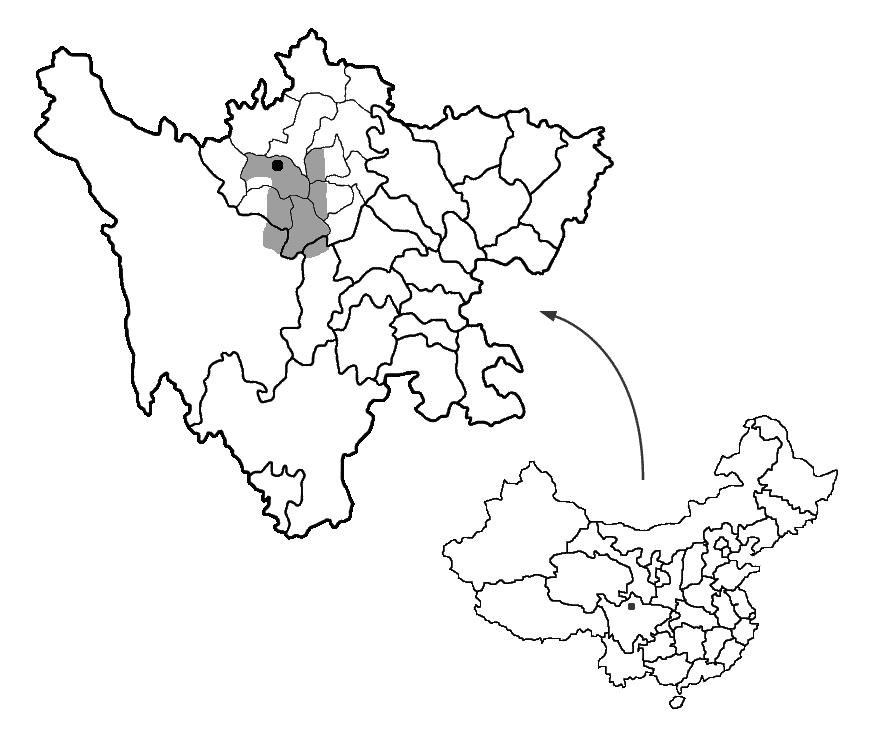
\includegraphics[height=100mm]{carte.JPG}
\caption{Rgyalrong languages}
\label{fig:rgyalrong}
\end{figure}

On the definition of the Rgyalrong and Rgyalrongic subgroups, see \citet{jackson00sidaba}.
 
In the present section, we first present a general overview of Japhug morphosyntax, then provide a list of all incorporating verbs, and finally analyse some their morphological and syntactic properties.

 \subsection{Overview of Japhug morphosyntax}
 Before studying incorporation in Japhug in detail, it is necessary to provide a general account of the main typological properties of that language.\footnote{The reader can also refer to  \citet{jackson03caodeng}, a sketch of Tshobdun, the closest relative of Japhug.}
 
 
 Japhug is a polysynthetic language, with obligatory person marking for two arguments with direct / inverse marking (on inverse marking in Rgyalrong languages see \citealt{delancey81direction},  \citealt{jackson02rentongdengdi} and  \citealt{jacques10inverse}). The verb distinguishes between singular, dual and plural, but not inclusive/exclusive. Transitivity (a feature of crucial importance for our study of incorporation) is marked by five distinct morphological processes:

 
 \begin{enumerate}
\item The aorist direct 3>3 prefix \ipa{a}--
\item The aorist 1/2sg>3 --\ipa{t} suffix (only occurs in open-syllable stem verbs)
\item The stem 3 formation, a stem alternation which occurs in direct 123sg>3 forms of verbs. The regular pattern is that verbs whose stem is in --\ipa{o}, --\ipa{u}, --\ipa{a} and --\ipa{ɯ} change to --\ipa{ɤm}, --\ipa{e}, --\ipa{e} and --\ipa{i} respectively.
\item The generic A form (which cannot occur on intransitive verbs).
\item The A participle which differs from the S participle by the addition of a possessive prefix correferent with the patient; compare the two phrases:
 \begin{exe}
\ex
\gll \ipa{kɯ-si}    \\
  \nmlz{}:S-die \\
 \glt  'The dead one'
 
\ex
\gll \ipa{ɯ-kɯ-sat}    \\
  3\sg{}-\nmlz{}:A-kill \\
 \glt  'The one who kills him.'

\end{exe}  

\end{enumerate} 
 
 Tense-Aspect-Modality is marked by a combination of several series of directional prefixes with vowel alternation on the verb root. The structure of the verbal word is more templatic than layered (following \cite[218]{bickel07inflectional}'s definition) and the basic template is the following:
 
   \begin{landscape}
\begin{table}[H]
\caption{The Japhug verbal template }\label{tab:template:derivational}
\begin{tabular}{llllll|llllllll|lllll} \toprule
 
\ipab{a-}  &  	\ipab{mɯ- }   &  	\ipab{ɕɯ-}   &\ipab{tɤ-} &  	\ipab{tɯ-}  &  	\ipab{wɣ-}   &

  	 \grise{\ipab{ʑɣɤ-}}  &  	\grise{\ipab{sɯ-}}  & \grise{\ipab{rɤ-}}& \grise{\ipab{nɤ-}} &   	 \grise{\ipab{a-}}   &  	\grise{\ipab{nɯ-}}  &  	\grise{\ipab{ɣɤ-}}  &  	\grise{\ipab{noun}}    &  	 \begin{math}\Sigma\end{math}    &  	\ipab{-a}  &  	\ipab{-t}  &  	\ipab{-nɯ}   &  \\
   &  	\ipab{mɤ-}   &  	\ipab{ɣɯ-}   &\ipab{pɯ-}&  	  &  	 
    & \grise{ }	  &  	 \grise{ }	  &  	  \grise{ }	  &  	   \grise{ }	&  	\grise{\ipab{sɤ-}}&  \grise{ }	 &  	\grise{\ipab{rɯ-}}  &  	 \grise{ }	  &  	  &  	  &  	  &  	\ipab{-ndʑi} &  \\
  &  	   &     &  etc.	  & & 	  &  	  &  	 & &  	  &  	 & &  etc.	  &  	  &  	  &  	  &  	  &  	  &  \\
1  &  	2  &  	3  &  	4  &  	5  &  	6  &  	7  &  	8  &  	9  &  	10  &  	11  &  	12  &  	13  &  	14  &  	15  & 16 &17&18\\
\bottomrule
\end{tabular}
\end{table}
\begin{multicols}{2}
\begin{enumerate}


\item Irrealis  \ipa{a}--, Interrogative \ipa{ɯ́}--, conative \ipa{jɯ}--
\item negation \ipa{ma}-- / \ipa{mɤ}-- / \ipa{mɯ}-- / \ipa{mɯ́j}--
\item \textbf{Translocative / Cislocative \ipa{ɕɯ}-- and \ipa{ɣɯ}--}
\item Directional prefixes (tɤ- pɯ- lɤ- thɯ- kɤ- nɯ- jɤ-, tu- pjɯ- lu- chɯ- ku- ɲɯ- ju-) permansive nɯ-, apprehensive ɕɯ-
\item Second person (\ipa{tɯ}--, \ipa{kɯ}-- 2>1 and ta- 1>2)
\item Inverse -\ipa{wɣ}- / Generic S/O prefix \ipa{kɯ}-, Progressive \ipa{asɯ}-. Note that the inverse is actually \textit{infixed} within the progressive as in \ipa{ɲɯ-tɯ-ɤ́<wɣ>sɯ-zgroʁ} \const{}-2-\textsc{prog}<\inv{}>-attach ``he is attaching you". 
\item Reflexive \ipa{ʑɣɤ}-- 
\item Causative \ipa{sɯ}--, Abilitative \ipa{sɯ}--
\item  Antipassive  \ipa{sɤ}-- / \ipa{rɤ}--
\item Causative sɯ-/z-/sɯɣ-/ɕɯ-/ɕ-/ɕɯɣ-/ʑ-/ɣɤ-, tropative \ipa{nɤ}--, applicative \ipa{nɯ}--
\item Passive or Intransitive thematic marker \ipa{a}-- / Deexperiencer \ipa{sɤ}--
\item Autobenefactive-spontaneous (appears in this position only when the passive/intransitive determiner is present, otherwise appears between positions 6 and 7) \ipa{nɯ}--
\item Other derivation prefixes \ipa{nɯ}-- \ipa{ɣɯ}-- \ipa{rɯ}-- \ipa{nɤ}-- \ipa{ɣɤ}-- \ipa{rɤ}--
\item Denominal / incorporated noun.  
\item Verb root 
\item Past 1sg/2sg transitive -\ipa{t} (aorist and evidential)
\item 1sg --\ipa{a}
\item Personal agreement suffixes (--\ipa{tɕi}, --\ipa{ji}, --\ipa{nɯ}, --\ipa{ndʑi})
\end{enumerate}


\end{multicols}
  \end{landscape}
Japhug and other Rgyalrong language are typologically unusual in being verb-final languages with mainly prefixing morphology. It is quite common to find a verb form with more than four or five prefixes in a row:
\begin{exe}
\ex
\gll \ipa{a-ɣɯ-lɤ-kɯ-sɯ-mtsʰam-a	}    \\
  \irr{}-\cisloc{}-\pfv{}:upstream-2>1-\caus{}-hear-1\sg{}   \\
 \glt  You will come  to tell me. (Japhug; The three sisters, 132)

\end{exe}  
 


 Derivational morphology is also extensive: both argument-promoting (causative, applicative, tropative), demoting (passive, antipassive, anticausative etc) and modal (abilitative, facilitative) derivations are attested and fairly productive (see for instance \citealt{jacques11demotion} or \citet{jackson06paisheng} on the related Tshobdun language).

Japhug is a strongly head-marking language, and its case marking system is rather poor: it only has an ergative clitic \ipa{kɯ}, an optional genitive  \ipa{ɣɯ} and an optional locative \ipa{zɯ}. Other grammatical relations are indicated by relational nouns with possessive prefixes (such as the dative --\ipa{ɕki}).

From the point of view of alignment typology, Japhug has ergative marking on nouns, tripartite alignment in relativization and  ergative alignment in generic marking (cf  \citealt{jacques11demotion}).

Japhug has a strong distinction between nouns and verbs, a feature, which as we have argued in section 2, is a prerequisite for the existence of incorporation. Nouns, unlike verbs, exhibit little morphology except possessive prefixes, whose paradigm is given in the following table, compared to the free pronouns (these prefixes also occur in some participial verb forms):

\begin{table}[H] \centering
\caption{Pronouns and possessive prefixes in Japhug}\label{tab:pronoun}
\begin{tabular}{lllllllll} \toprule
 Free pronoun & Prefix & \\
\midrule
 \ipa{aʑo},     &	\ipa{a--}  &		1\sg{} \\
\ipa{nɤʑo},  &	\ipa{nɤ-}  &			2\sg{} \\
\ipa{ɯʑo}  &	\ipa{ɯ-}  &			3\sg{} \\
\ipa{tɕiʑo}  &	\ipa{tɕi-}  &			1\du{} \\
\ipa{ndʑiʑo}  &	\ipa{ndʑi-}  &		2\du{} \\	
\ipa{ʑɤni}  &	\ipa{ndʑi-}  &		3\du{} \\	
\ipa{iʑo}   &	\ipa{i-}  &			1\pl{} \\
\ipa{nɯʑo}   &	\ipa{nɯ-}  &			2\pl{} \\
\ipa{ʑara}  &	\ipa{nɯ-}  &			3\pl{} \\
\bottomrule
\end{tabular}
\end{table}
 Some intrinsically possessed noun, especially body parts, kinship terms and relational nouns, must appear with either possessive prefix or the indefinite possessive \ipa{tɯ}-- or \ipa{tɤ}--.

%In this section, we will study in detail the morphological and syntactic properties of incorporation in Japhug. First, we will provide a complete list of all the examples of incorporation discovered in our fieldwork; although this morphological process is still productive, as it applies to loanwords, it is by no means common and examples are limited in number. Second, we will describe the morphological properties of the incorporated verbs, in particular the bound form of the nouns and the presence of derivational prefixes. Third, we will discuss some of the syntactic and semantic properties of incorporating verbs.

 \subsection{Incorporating verbs in Japhug} \label{subsec:incorp.list}
Japhug presents some verbs that can be described as incorporating according to the definition given in section 2: verbs non restricted to non-finite forms whose stem contains a verbal and a nominal root, both of which appear independently.

 Unlike other derivational processes, incorporating verbs are not very many in Japhug: only  35 have been discovered up to now. Although incorporation is fairly rare in traditional stories, these examples show that this process is still productive, as it applies not only to native vocabulary, but also to Tibetan (\ipa{fsoʁ} ``earn'' < Tibetan \textit{bsogs}), \ipa{ɯ-ɲɤm} ``flesh'' < \textit{nyam}) and Chinese (\ipa{tʂʰa} ``tea'' \zh{茶} chá, \ipa{pɕawtsɯ} ``money'' \zh{票子} piàozi) loanwords. Chinese loanwords are almost all extremely recent, dating from after 1950.



In the following table, nouns roots in incorporating verbs are written in bold, and separated from other morphemes by a hyphen. For each incorporating verb, we give the base noun and verb from which it is built. Note that some of the nouns are intrinsically possessed nouns, and must appear with a possessive prefix (here systematically given as the third person \ipa{ɯ}--) or the indefinite possessive \ipa{tɯ}--.  


Verbs for which we have indicated \ipa{idiom} as the meaning only appear in noun-verb collocations with the same noun as in the incorporating verb. For instance \ipa{tɯ-ʑi} \ipa{loʁ} is an idiom meaning ``have nausea'':
 \begin{exe}
\ex
\gll  \ipa{ɯʑo} \ipa{ɯ-ʑi} \ipa{ɲɯ-loʁ}  \\
 he 3\sg{}.\poss{}-nausea \const{}-have.nausea \\
 \glt He has nausea. (elicitation, Dpalcan)
\end{exe}  
Neither  the noun \ipa{tɯ-ʑi} nor the verb \ipa{loʁ} can appear on their own, though they behave morphologically like independent words. 
 
The morphological and morphosyntactic properties of these incorporating verbs will be analysed in the next sub-sections.
  \begin{landscape}
  
  \begin{table}[h]
  \caption{Examples of incorporation in Japhug}\label{tab:incorp.japhug}
\begin{tabular}{lllllllll}
%\begin{longtable}{lllllllll}

   \toprule
base noun & meaning & base verb & meaning & incorporating verb & meaning \\
\midrule
 \ipa{tɯ-ku} & head & \ipa{amtɕoʁ} & pointed (vs)& \ipa{a-\textbf{kɤ}-mtɕoʁ} & with a pointed head \\
 \ipa{cʰa} & alcohol & \ipa{tsʰi} & drink (vt)& \ipa{ɣɯ-\textbf{cʰɤ}-tsʰi } & to drink alcohol\\
  \ipa{cɯ} & stone & \ipa{pʰɯt} & take out, cut down (vt) & \ipa{ ɣɯ-\textbf{cɯ}-pʰɯt } & to take out stones (out of the field)\\
   \ipa{tɯ-ɣli} & dung & \ipa{tɕɤt} & take out (vt)& \ipa{ɣɯ-\textbf{ɣlɯ}-tɕɤt} & to take out dung (out of the stable, \\
   &&&&&    to make fertilizer)\\
   
  \ipa{ɣndʑɤβ} & fire (big) & \ipa{ta} & put (vt)& \ipa{ɣɯ-\textbf{ɣndʑɤβ}-ta} & to clear (fields) with fire  \\
  \ipa{kʰɯna} & dog & \ipa{tsʰoʁ} & attach (vt) & \ipa{ɣɯ-\textbf{kʰɯ}-tsʰoʁ} & to turn the dog loose on   \\
  \ipa{pɕawtsɯ} & money & \ipa{fsoʁ} & earn & \ipa{ɣɯ-\textbf{pɕawtsɯ}-fsoʁ} & to earn money  \\
    \ipa{tɯ-rɟɯ} & riches & \ipa{fsoʁ} & earn & \ipa{ɣɯ-\textbf{rɟɯ}-fsoʁ} & to earn riches  \\
  \ipa{si} & tree, wood & \ipa{pʰɯt} & take out, cut down (vt) &   \ipa{ɣɯ-\textbf{sɯ}-pʰɯt} & to cut wood (to make firewood) \\
  \ipa{tʂʰa} & tea & \ipa{tsʰi} & drink (vt)& \ipa{ɣɯ-\textbf{tʂʰɤ}-tsʰi} & to have tea  \\
  \ipa{tʂu} & way & \ipa{mtsʰi} & lead (vt)& \ipa{ɣɯ-\textbf{tʂɤ}-mtsʰi} & to lead the way  \\
  \ipa{tɤ-jlɤβ} & steam & \ipa{sqa} & cook (vt) & \ipa{nɤ-\textbf{jlɤβ}-sqa} & to cook with steam  (vt) \\
  
  \ipa{tɯ-ku} & head & \ipa{tɕʰɯ} & gore (vt)  & \ipa{nɤ-\textbf{kɤ}-tɕʰɯ} & to hit with the head (vt)  \\
    \ipa{tɯ-zgrɯ} & elbow & \ipa{tɕʰɯ} & gore (vt)  & \ipa{nɯ-\textbf{zgrɯ}-tɕʰɯ} & to hit with the elbow (vt)  \\
   \ipa{ɯ-mpʰru} & one after the other & \ipa{ʑa} & start (vt) & \ipa{nɤ-\textbf{mpʰru}-ʑa} & to do after after the other  \\
  \ipa{tɤ-pʰɯ} & clod (of earth) & \ipa{xtsɯ} & pound (vt)& \ipa{nɤ-\textbf{pʰɯ}-xtsɯ} & to break clods of earth  \\
   \ipa{ɯ-qa} & root & \ipa{ʑa} & start (vt) &\ipa{nɤ-\textbf{qa}-ʑa} & to start from the beginning (vt)  \\
  \ipa{ɯ-qʰu} & back, behind & \ipa{ru} & look & \ipa{nɤ-\textbf{qʰa}-ru} &to  look back  \\

  \ipa{ɯ-qʰu} & back, behind  & \ipa{ŋga} & wear (vt)& \ipa{nɤ-\textbf{qʰɤ}-ŋga} & to wear on the back  \\
   \ipa{tɯ-ʑi} & nausea & \ipa{loʁ} & (idiom) & \ipa{nɤ-\textbf{ʑɯ}-loʁ} & to have nausea  \\
   
   
  \ipa{jla} & hybrid yak & \ipa{lɤɣ} & herd (vl) & \ipa{nɯ-\textbf{jlɤ}-lɤɣ} & to herd hybrid yaks   \\
  \ipa{jla} & hybrid yak & \ipa{mtsʰi} & lead (vt) & \ipa{nɯ-\textbf{jlɤ}-mtsʰi} & to lead hybrid yaks  \\
  \ipa{mbro} & horse & \ipa{rɟɯɣ} & run & \ipa{nɯ-\textbf{mbrɤ}-rɟɯɣ} & to gallop  \\
  \ipa{tɯ-nŋa} & debt & \ipa{tʂo} & pay & \ipa{nɯ-\textbf{nŋɤ}-tʂo} & to pay back one's debt  \\   



 \end{tabular} 
\end{table}      
         
     \begin{table} [h] 
\begin{tabular}{lllllllll}         
      \ipa{ɯ-ɲɤm} & flesh & \ipa{kʰe} & (idiom) & \ipa{nɯ-\textbf{ɲɤm}-kʰe} & to be skinny    \\ 
      \ipa{ɯ-ɲɤm} & flesh & \ipa{sɯ} & plump & \ipa{nɯ-\textbf{ɲɤm}-sɯ} & to be plump    \\ 
      
        \ipa{paʁ} & pig & \ipa{lɤɣ} & herd (vl) & \ipa{nɯ-\textbf{paʁ}-lɤɣ} & to herd pigs    \\ 
    \ipa{ɯ-pʰaʁ} & side & \ipa{ɲɤl} & (not independent) & \ipa{nɯ-\textbf{pʰaʁ}-ɲɤl} & to lay on the side    \\ 
       \ipa{ɯ-qʰu} & behind & \ipa{astu} & straight & \ipa{nɯ-qʰɤ-stɯ-stu} & to back up    \\       
           \ipa{tɯ-rma} & household & \ipa{kro} & share & \ipa{nɯ-\textbf{rmɤ}-kro} & to split the household   \\ 
                  \ipa{tɤ-rme} & hair & \ipa{mbe} & old & \ipa{nɯ-\textbf{rmɤ}-mbe} & to moult  \\                    
        \ipa{tɯ-sni} & heart & \ipa{ɲaʁ} &black & \ipa{nɯ-\textbf{snɯ}-ɲaʁ} &   to harm \\                   
   \ipa{zrɯɣ} & louse & \ipa{ru} &look & \ipa{nɯ-\textbf{zrɯɣ}-ru} &   to look for lice \\                           
     \ipa{tʂu} & road & \ipa{sti} &block & \ipa{nɯ-\textbf{tʂɤ}-qɤ-sti} &  to block the way  \\                           
  \ipa{tɯ-mbrɯ} & anger & \ipa{ŋgɯ} &(idiom) & \ipa{sɤ-\textbf{mbrɯ}-ŋgɯ} &  to be detestable \\                           
        \ipa{tɯ-ʑi} & nausea & \ipa{loʁ} & (idiom) & \ipa{sɤ-\textbf{ʑɯ}-loʁ} & to be disgusting \\
\bottomrule
 \end{tabular} 
\end{table} 
  \end{landscape}
Beside the 34 examples above, a special case must be made of the verb \ipa{kɤtɯpa} ``to speak''. This verb   etymologically includes the verbal root \ipa{--pa}, originally meaning ``to do'', but restricted in modern Japhug to the meaning ``to close (the door)'' or as a light verb with ideophones. The first part \ipa{kɤtɯ}-- is an ablauted form of \ipa{kɤ-ti} the patient participle of the verb \ipa{ti} ``to say'' and literally means ``the things that are said'' (in some contexts it also means ``niggling''). The verb \ipa{kɤtɯpa} is only a fringe case of incorporation, as the incorporated element is itself the nominalized form of a verb.\footnote{The noun  \ipa{ɣndʑɤβ} ``devastating fire'' in \ipa{ɣɯ-ɣndʑɤβ-ta} ``to clear with fire'' is another such case, but unlike \ipa{kɤtɯpa}, the incorporated form is a nominalized verb only etymologically, as  \ipa{ɣndʑɤβ} is an non-productive and synchronically opaque nominalized form, while  \ipa{kɤ-ti} is a regular form that follows the productive pattern. } 

 
  
  
 This verb is defective, and only occurs in non-past first and third person forms. It is morphologically transitive, and undergoes --\textit{a} > --\textit{e} ablaut in singular forms. The following table compares the non-past (direct, i.e. with a third person patient) forms of the transitive verb \ipa{ndza} ``to eat'' with those of  \ipa{kɤtɯpa}:

\begin{table}[H] \centering
\caption{Paradigm of the verb  \ipa{kɤtɯpa} ``to speak''}\label{tab:katWpa}
\begin{tabular}{lllllllll} \toprule
Person & ``to eat'' & ``to speak'' & \\
\midrule
1\sg{} &  \ipa{ndze-a}& \ipa{kɤtɯpe-a} \\
		2\sg{} &  \ipa{tɯ-ndze}& XX \\
		3\sg{} &  \ipa{ndze}& \ipa{kɤtɯpe} \\
	1\du{} &  \ipa{ndza-tɕi}& \ipa{kɤtɯpa-tɕi} \\
2\du{} &  \ipa{tɯ-ndza-ndʑi}& XX  \\
	3\du{} &  \ipa{ndza-ndʑi}& \ipa{kɤtɯpa-ndʑi} \\
	1\pl{} &  \ipa{ndza-j}& \ipa{kɤtɯpa-j} \\
		2\pl{}&  \ipa{tɯ-ndza-nɯ}& XX  \\
			3\pl{} &  \ipa{ndza-nɯ}& \ipa{kɤtɯpa-nɯ} \\
\bottomrule
\end{tabular}
\end{table}
The non-past being the only tense which is not prefixed in Japhug, we observe that the only attested forms of this verbs are precisely those which are not   prefixed; in other word, the verb \ipa{kɤtɯpa} ``to speak'' is one of the few verbs in the language (alongside the highly irregular \ipa{ɣɤʑu} ``to be there'' and \ipa{maŋe} ``not to be there'') which cannot appear with any prefix.
  
Given the peculiarities of the verb \ipa{kɤtɯpa} ``to speak'', it will not be treated in the following discussion on incorporation, as it constitutes a case different from all other true incorporating verbs.
  

%vi vt vl vs
   \subsection{Morphological  properties}
   All incorporating verbs in Japhug  except \ipa{kɤtɯpa} ``to speak'' exhibit a very strict morphological structure, which we can represent as follows:
   
   \begin{tabular}{IIII}
\textsc{derivation prefix} & \textsc{incorporated noun} & \textsc{verbal stem} \\
\ipa{nɯ}--, \ipa{nɤ}--, \ipa{ɣɯ}--, \ipa{sɤ}-- && \\
\end{tabular}

The nature of the derivation prefixes will be studied in more detail in section \ref{sec:denom}.    A few examples such as \ipa{nɯtʂɤqɤsti} ``to block the way'' present more than one incorporated element, but we will first restrict the discussion to this basic structure.
 
The incorporated noun undergoes two main changes. First, in the case of possessed noun prefixes with either the indefinite possessive prefix \ipa{tɯ}-- / \ipa{tɤ}-- or the third person prefix \ipa{ɯ}--, this prefix disappears in the incorporated form of the noun. Second, in open-syllable nouns, the vowel undergoes a series of regular changes, which we call the \ipa{status constructus}:

\begin{table}[H] \centering
\caption{Status constructus}\label{tab:etatconstruit} 
\begin{tabular}{lllllllll} \toprule
basic noun  & incorporated noun &\\
 --\ipa{a} & --\ipa{ɤ} / --\ipa{a} \\
  --\ipa{o} & --\ipa{ɤ} / --\ipa{a} \\
    --\ipa{e} & --\ipa{ɤ} / --\ipa{a} \\
  --\ipa{u} & --\ipa{ɤ} / --\ipa{a} \\
   --\ipa{i} & --\ipa{ɯ} \\
    \bottomrule
\end{tabular}
\end{table}

The \ipa{status constructus} of some nouns is  irregular, in particular the noun ``dog'' \ipa{kʰɯna} which becomes \ipa{kʰɯ}-- instead of expected *kʰɯnɤ-. Not only possessive prefixes are lost during derivation, but also derivational prefixes as in \ipa{tɯ-nŋa} ``debt'' a noun derived from \ipa{nŋa} ``owe'' by the action nominalization prefix \ipa{tɯ}--. The only case of a prefix preserved in the construct state in the list is that of \ipa{ɣndʑɤβ} ``fire''. This noun is an irregular nominalization of \ipa{ndʑɤβ} ``to burn (vi)'', an anticausative derivation of the transitive \ipa{tɕɤβ} ``burn (vt)''. The regular form \ipa{kɯ-ndʑɤβ} is also attested; \ipa{ɣ}-- originates from \ipa{kɯ}-- by syncope (a cluster such as /kndʑ/ would be impossible in Japhug). Since this \ipa{ɣ}--  is not felt synchronically as a prefix anymore, it is not suppressed during incorporation.

The \ipa{status constructus} is not limited to incorporating verbs, but also occurs in nominal compounds:


\begin{table}[H] \centering
\caption{Examples of noun compounds with status constructus}\label{tab:nom.comp}
\begin{tabular}{lllllllll} \toprule
Element 1 & meaning  & Element 2 & meaning & compound noun & meaning \\
  \ipa{tɯ-ku} & head & \ipa{tɤ-rme} & hair & \ipa{tɯ-kɤ-rme} & hair (on the head) \\
  \ipa{tʂu} & road & \ipa{tɤ-mtʰɯm} & meat & \ipa{tʂɤ-mtʰɯm} & provision of\\
  &&&&& meat for the road \\
 \bottomrule
\end{tabular}
\end{table}
 The first element is always a noun in \ipa{status constructus}, and the second element undergoes little change, except for  the loss of possessive prefixes.
   
   
The presence of a distinct bound form for incorporated nouns, and the fact that this bound form also occurs in nominal compounds, are characteristics also attested in many languages with incorporation, in particular the Algonquian examples discussed in section 2.
 
   
 
 
   
  \subsection{Syntactic properties}
Incorporating verbs are not common in traditional stories, so that a detailed study of the function of this construction is difficult. 

The incorporated noun cannot be modified by either stranded demonstratives or adjectives as in languages such as Hopi (see for instance \citealt[121]{haugen08incorp}), and it is never referential. Although incorporation retains some degree of productivity, attempts at creating new incorporating verbs on the model of the ones discovered in the stories met with disagreement by the speakers. For instance, while \ipa{nɯ-jlɤ-lɤɣ} ``herd hybrid yaks'' and \ipa{nɯ-paʁ-lɤɣ} ``herd pigs'' are possible, it is impossible (or at least not fully acceptable) to produce a verb such as *nɯ-qaʑɤ-lɤɣ ``herd sheep'', probably because such an activity is not in Rgyalrong culture ``recognized sufficiently often to be considered name-worthy in its own right'', as \citet[848]{mithun84incorp} puts it.


The incorporated noun can have three functions:

 \begin{exe}
\ex
 \glt  O of a transitive verb. \ipa{ɣɯ-\textbf{sɯ}-pʰɯt} ``cut wood''.
  \glt  S of an  intransitive  verb. \ipa{a-\textbf{kɤ}-mtɕoʁ} ``have a pointed head''.
 \glt Adjunct. \ipa{nɤ-\textbf{qʰa}-ru} ``look back''.
\end{exe}   
Note that no examples of incorporated A have been discovered: Japhug follows the well-known implicational hierarchy, according to which ``if a language incorporates nouns in just one function, they will be direct objects;
if a language incorporates only two types of arguments, they will be direct
objects and subjects of intransitive verbs" (\citealt[19]{aikhenvald07wordformation}).


When the O is incorporated, the  incorporating verb becomes intransitive: this is a case of saturating incorporating (type I incorporation according to  \citet{mithun84incorp}'s hierarchy). Compare the two following forms competing constructions:


 \begin{exe}
\ex \label{ex:incorp.debt}
\gll  \ipa{nɯ-nɯ-\textbf{nŋɤ}-tʂo-a} \\
\aor{}-\textsc{derivation}-\textbf{debt}-pay-1\sg{} \\
\ex \label{ex:n.incorp.debt}
\gll \ipa{a-nŋa}  \ipa{nɯ-tʂo-t-a} \\
1\sg{}.\poss{}-debt \aor{}-pay-\pst{}-1\sg{} \\
 \glt I paid my debt.
\end{exe}   

In example \ref{ex:n.incorp.debt} without incorporation, the verb \ipa{tʂo} ``to pay'', is transitive, as shown the presence of the past suffix --\ipa{t}, which only occurs in 1\sg{}>3 and 2\sg{}>3 forms of transitive verbs. In the corresponding construction with incorporation in example \ref{ex:incorp.debt}, the verb cannot appear with this suffix --\ipa{t}, showing that it was intransitivized by the process of incorporation.

When the S is incorporated, the verb remains intransitive, and interestingly the free equivalent of the incorporated noun can in at least one example appear as the S (\ipa{tɯ-ku} ``head'' becomes --\ipa{kɤ}-- in \textit{status constructus}):
 \begin{exe}
\ex
\begin{xlist}[(ii)]
\exi{(i)} 
\gll  \ipa{ɯ-\textbf{ku}} \ipa{ɲɯ-ɤmtɕoʁ}  	  \\
 3\sg{}-\textbf{head} \const{}-pointed\\
\exi{(ii)} 
\gll  \ipa{ɯ-\textbf{ku}} \ipa{ɲɯ-ɤ-\textbf{kɤ}-mtɕoʁ}  	  \\
 3\sg{}-\textbf{head} \const{}-\textsc{derivation}-\textbf{head}-pointed\\
 \glt Its head is pointed (of a knife). (elicitation, Dpalcan)
 \end{xlist}
\end{exe}   

When an adjunct is incorporated, the verb  remains transitive in some cases, as in \ipa{nɤkɤtɕʰɯ} ``hit with the head:
  \begin{exe}
\ex
\gll  \ipa{kɤ́-wɣ-nɤ-\textbf{kɤ}-tɕʰɯ-a}  	  \\
 \aor{}-\inv{}-\textsc{derivation}-\textbf{head}-gore-1\sg{} \\
 \glt He hit me with the head. (elicitation, Dpalcan)
\end{exe}   

However we have found no case of Mithun's type II incorporation, when a verb incorporating an O argument remains transitive, and promotes an adjunct to O role.

Although the meaning of some of the incorporating verbs is not compositional, that is one cannot guess the exact meaning of the verb from that of the incorporated noun and the verb, some incorporating verbs are quite transparent in this regard. This is for instance the case of \ipa{ɣɯ-pɕawtsɯ-fsoʁ} ``earn money'', a recent incorporating verb since it contains a Chinese loanword.

We find the two following examples a few sentences away in the same story:


 
 
 
 \begin{exe}
\ex
\gll    	\ipa{ɬasa} 	\ipa{ju-kɯ-ɕe} 		\ipa{tɕe,} 	\ipa{nɯtɕu}  \ipa{pɕawtsɯ} \ipa{kɤ-fsoʁ} 	\ipa{ɲɯ-mbat} \\
Lhasa	\textsc{ipf}-\textsc{genr}:S/O-go \coord{} there money \inftv{}-earn \const{}-easy \\
 \glt ‘If one goes to Lhasa, money is easy to earn there.’ (Lobzang, 22)
\end{exe}   
 
 \begin{exe}
\ex
\gll    	\ipa{nɤ-mbro} 	\ipa{nɤ-rŋɯl} 	\ipa{tu-rke-a} 		\ipa{tɕe} \ipa{kɯ-ɣɯ-pɕawtsɯ-fsoʁ} 			\ipa{jɤ-ɕe} 	\ipa{tɕe} \\
2\sg{}.\poss{}-horse	2\sg{}.\poss{}-silver	\ipf{}-put.in[3]-1\sg{}	\coord{} \nmlz{}:S/A-\textsc{derivation}-money-earn	\imp{}-go	\coord{} \\
 \glt ‘I will prepare a horse and some silver for you, go to earn money.’ (Lobzang, 17)
\end{exe}   
In the first example, \ipa{pɕawtsɯ} ``money'' is the free object of the transitive verb \ipa{fsoʁ} ``earn''. In the second sentence, we find the corresponding incorporating verb. In both cases, the Noun-Verb construction and the incorporated verb could have been substituted one for the other without noticeable change of meaning.
 
Interestingly, an important proportion (more than half) of textual examples of compositional incorporated verbs such as these come from non-finite verbal forms, especially as complement of movement verbs: 
 \begin{exe}
\ex
\gll    	\ipa{tɯ-sŋi}	\ipa{ci} \ipa{zɯ}	\ipa{nɯ},	\ipa{tɤ-tɕɯ}	\ipa{nɯ}	\ipa{li}	\ipa{kɯ-ɣɯ-sɯ-pʰɯt}	\ipa{lɤ-ari}	\ipa{ɲɯ-ŋu}, \\
  one-day \textsc{indef} \loc{} \topic{} \neu{}-boy \topic{} again \nmlz{}:S/A-\textsc{derivation}-wood-chop \aor{}:\textsc{upstream}-go[II]  \const{}-be\\
 \glt `One day, the boy went again to chop wood.' (The demon, 7)
\end{exe} 
 
These incorporating  verbs differ from constructions such as English \ipa{go berry-picking}, as they can be fully conjugated, but the prevalence of these verbs in non-finite forms in spontaneous speech deserves a more detailed study. More traditional stories and conversations need to be collected in order to have enough examples to be able to undertake meaningful statistical studies, due to the rarity of these forms in natural speech.
 
\section{Denominal derivation in Japhug} \label{sec:denom}

%+ Antipassicv  tɯ-pɣaʁ > rɤ-pɣaʁ tɯ-krɤz > rɤkrɤz
%autre article


Japhug has a very rich system of denominal derivations, which cannot be treated exhaustively in the scope of this paper. All denominal verbs are derived from nouns by means of a derivation prefix. The attested prefixes are the following:

\begin{table}[H] \centering
\caption{List of denominal prefixes in Japhug}\label{tab:denom.pref} 
\begin{tabular}{lllllllll} \toprule
Form& Property \\
\midrule
\ipa{nɯ}--, \ipa{nɤ}-- & intransitive and transitive \\
\ipa{rɯ}--, \ipa{rɤ}-- & intransitive and transitive \\
\ipa{ɣɯ}--, \ipa{ɣɤ}-- & intransitive and transitive \\
\ipa{sɯ}--  & transitive verb with instrument, intransitive verb of position \\
\ipa{mɤ}-- & transitive verb with body part, intransitive verb of position \\
\ipa{sɤ}-- & intransitive verb (property) \\
\ipa{aɣɯ}-- & intransitive verb (property) \\
    \bottomrule
\end{tabular}
\end{table}

Many denominal verbs are derived from intrinsically possessed nouns, which always bear either a possessive prefix or an indefinite possessor prefix \ipa{tɯ}-- or \ipa{tɤ}--. The vocalism /ɯ/ or /ɤ/ of the denominal prefixes on whether the base noun has \ipa{tɯ}-- or \ipa{tɤ}--, though there are a few exceptions. For instance, out of \ipa{tɤ-ʑri} ``dew'' one can derive \ipa{nɤ-ʑri} ``be covered with dew'' (vi), while out of \ipa{tɯ-ʑɯβ} ``sleep (n)'' one derives \ipa{nɯ-ʑɯβ} ``sleep (vi)''. However, numerous exceptions to this general principle exist; in particular, the vowel /ɯ/ tends to /ɤ/ next to a uvular consonant.


There are several pairs where \ipa{nɯ}-- / \ipa{nɤ}-- derives a transitive verb while \ipa{rɯ}--/ \ipa{rɤ}-- derives an intransitive one, such as \ipa{tɯ-krɤz} ``discussion'' > \ipa{nɯkrɤz} ``discuss (vt)'' vs. \ipa{rɤkrɤz} ``discuss (vi)''.

However, the transitivity of the derived verb is not always predictable from the form of the prefix. The following table illustrates the transitivity of the denominal verbs depending on their derivational prefix in our Japhug unpublished dictionary:


\begin{table}[H] \centering
\caption{Proportion of transitive and intransitive verbs}\label{tab:denom.pref2} 
\begin{tabular}{lllllllll} \toprule
Form& Property \\
\midrule
		&	vi	&	vt	\\
\ipa{nɯ}--,	\ipa{nɤ}--	&	44	&	46	\\
\ipa{rɯ}--,	\ipa{rɤ}--	&	28	&	4	\\
\ipa{ɣɯ}--,	\ipa{ɣɤ}--	&	6	&	8	\\
\ipa{sɯ}--		&	2	&	5	\\
\ipa{mɤ}--		&	2	&	3	\\
\ipa{sɤ}--		&	2	&		0\\
\ipa{aɣɯ}--		&	12	&	0	\\
    \bottomrule
\end{tabular}
\end{table}
Discussing in detail the semantic properties of each prefix would require considerable space and will not be attempted in this paper. We will only focus on the functions of the four forms which are common between denominal verbs and incorporating verbs: \ipa{nɯ}--, \ipa{nɤ}--, \ipa{ɣɯ}--, \ipa{sɯ}-- and \ipa{sɤ}--

The prefix \ipa{nɯ}-- and its variant \ipa{nɤ}-- appear in a considerable variety of verbs, as illustrated by the following table:

\begin{table}[H] \centering
\caption{Examples of the denominal prefix \ipa{nɯ}--}\label{tab:denom.pref.nW} 
\begin{tabular}{lllllllll} \toprule
Base noun& Meaning & Derived verb & Meaning & \\
\midrule
\ipa{ɯ-pʰɯ} &prince & \ipa{nɯ-pʰɯ} & to be of a correct price&vi, stative\\
\ipa{sɣa} &rust & \ipa{nɯ-sɣa} &to be rusty &vi, stative\\
\ipa{qaɟy} &fish & \ipa{nɯ-qaɟy} &to fish &vi\\
\ipa{tɯ-ŋgra} &salary & \ipa{nɯ-ŋgra} &to receive a salary &vi\\
\ipa{mtʰɯ} & spell& \ipa{nɯ-mtʰɯ} &to cast a spell &vt\\
\ipa{kɯjŋu} & oath& \ipa{nɯ-kɯjŋu} &to swear &vt\\
\ipa{mbɯrlɤn} &plane & \ipa{nɯ-mbɯrlɤn} &to plane    &vt\\
\ipa{smɤn} &medecine & \ipa{nɯ-smɤn} &to treat    &vt\\
\ipa{mkɤɣɯr} &necklace & \ipa{nɯ-mkɤɣɯr} &to wear as a necklace    &vt\\
\ipa{tɯ-rdoʁ} &a piece & \ipa{nɯ-rdoʁ} &to pick up piece by piece & vt\\
\ipa{ʁjoʁ} & servant& \ipa{nɯ-ʁjoʁ} & to give orders to&vt\\
\ipa{ʁgra} & enemy& \ipa{nɯ-ʁgra} & to treat as an enemy&vt\\
\ipa{tɯ-skʰrɯ} &body  & \ipa{nɯ-skʰrɯ} &to be pregnant of &vt\\
    \bottomrule
\end{tabular}
\end{table}
The prefix  \ipa{nɯ}-- can derive four major types of verbs, though some (such as ``to be pregnant'') cannot be easily classified into any category:
	First, intransitive stative verbs denoting a property related to the base noun, as in ``to be rusty'' and ``to be of a correct price''.
	
	Second, intransitive verbs describing an activity whose purpose is to obtain the entity designated by the base noun, as in ``to fish'' or ``to receive a salary''; the meaning is never ``to make X'' or ``to become X''.
	
	Third, transitive action verbs derived from instrument nouns (as in ``to plane'' or ``to treat'').
	
	Fourth, transitive verbs meaning ``to consider as, to treat as'' relative to the base noun.

%The prefixes \ipa{sɤ}-- and \ipa{aɣɯ}-- exclusively derives stative verb expressing a property of the noun, such as \ipa{tɤ-ndɤɣ} ``poison'' > \ipa{sɤ-ndɤɣ} ``be poisonous''.

The prefix \ipa{ɣɯ}-- is much less common than \ipa{nɯ}--. The following example illustrate its main functions:
\begin{table}[H] \centering
\caption{Examples of the denominal prefix \ipa{ɣɯ}--}\label{tab:denom.pref.GW} 
\begin{tabular}{lllllllll} \toprule
Base noun& Meaning & Derived verb & Meaning & \\
\midrule
\ipa{tɤ-tsrɯ} &sprout & \ipa{ɣɤ-tsrɯ} & to sprout&vi\\
\ipa{ɕoŋtɕa} &timber & \ipa{ɣɯ-ɕoŋtɕa} & to chop timber &vi \\
\ipa{tɯ-tɕʰa} & message & \ipa{ɣɯ-tɕʰa} & to answer &vt \\
\ipa{ɕkat} &load & \ipa{ɣɯ-ɕkat} & to load (an animal) &vt \\
\ipa{tɤ-fkɯm} &bag & \ipa{ɣɯ-fkɯm} & to put in a bag &vt \\
    \bottomrule
\end{tabular}
\end{table}
The allomorph \ipa{ɣɤ}-- only occurs with intransitive verbs expressing the generation of the entity designated by the base noun (as in ``to sprout''). Some uses of \ipa{ɣɯ}-- seem to be identical to that of \ipa{nɯ}--. For instance, the case for ``to chop timber''  is similar to that observed with the verb \ipa{nɯ-qaɟy} ``to fish'' above. Verbs such as \ipa{ɣɯ-ɕkat} ``to load'' and \ipa{ɣɯ-fkɯm} ``to put in a bag'' on the other hand exemplify a type of derivation slightly different from that of \ipa{nɯ}--, meaning especially ``to put in a container'', the container being the base noun.


The prefix \ipa{sɯ}-- appears in two cases. First, with body parts or instrument, where it derives a labile or a transitive verb expressing the action of that instrument (\ipa{tɯ-jaʁndzu} ``finger'' > \ipa{sɯ-jaʁndzu} ``show with the finger''). Second, with  with nouns expressing a position such as \ipa{ndzɯpe} ``way of sitting (without crossing legs, the way women sit in the traditional society) > \ipa{sɯ-ndzɯpe} ``sit (without crossing legs, vi)''.

  
  
  
\subsection{Deexperiencer / tropative pairs}
Aside from the three groups of prefixes \ipa{nɯ}--/ \ipa{nɤ}--, \ipa{ɣɯ}-- and  \ipa{sɯ}-- discussed above, we must mention the case of the deexperiencer / tropative pairs in \ipa{sɤ}-- / \ipa{nɤ}-- (see table \ref{tab:deexperiencer} for examples of these prefixes), in relation to the pair of incorporating verbs \ipa{sɤ-\textbf{ʑɯ}-loʁ} ``to be disgusting'' and \ipa{nɤ-\textbf{ʑɯ}-loʁ} ``to have nausea'' derived from the collocation     \ipa{tɯ-ʑi}  \ipa{loʁ} ``to have nausea''.


Apart from these two verbs, we find three pairs of verb which present the same apparent meaning derivation: 

\begin{table}[H]
\caption{Deexperiencer / Tropative pairs } 
\begin{tabular}{lllllllll} \toprule
 
Deexperiencer 	&Meaning	&Tropative 	&Meaning &Noun	&Meaning\\

verb && verb\\
\midrule
\ipa{sɤ-re}  &	to be ridiculous 	& \ipa{nɤ-re}  &	  to laugh (labile) &\ipa{tɤ-re}  &	  laughter\\
\ipa{sɤ-mtsʰɤr}  &	to be strange 	& \ipa{nɤ-mtsʰɤr}  &	  to consider (vt)  &\ipa{tɤ-mtsʰɤr}  &	 strange\\

&&& to be strange && event \\
\ipa{sɤ-ŋɤβ}  &	to be such that   	& \ipa{nɤ-ŋɤβ}  &	  to feel sorry  (vt) & \\
& people do \\
&not want it  \\
\bottomrule
\end{tabular}
\end{table}
The verb  \ipa{nɤ-re} is labile, meaning ``to laugh at (someone)'' when used transitively, and ``to laugh'' when used intransitively.

The first two verb pairs \ipa{sɤ-re} / \ipa{nɤ-re} and  \ipa{sɤ-mtsʰɤr} / \ipa{nɤ-mtsʰɤr} are similar, related to base nouns prefixed in \ipa{tɤ}--. Note that the prefix in these nouns is the indefinite possessive, which disappears when a possessive prefix is added:
 \begin{exe}
\ex
\gll  \ipa{ɯ-re} 	\ipa{ci} 	\ipa{ɕmɯɣ} 	\ipa{ɲɤ-ɕlɯɣ,}   \\
 3\sg{}.\poss{}-laughter a.little   \textsc{ideo}:1:laughter \evd{}-drop \\
 \glt She (could not resist and) laughed a little.  (The Frog, 100)
\end{exe}   

For the pair \ipa{sɤŋɤβ} / \ipa{nɤŋɤβ} on the other hand, no corresponding noun seem to exist, though it could have existed or be attested in other varities of Japhug.

  
The nature of the derivation in the case of these pairs is intriguing, as they would seem to exemplify the deexperiencer and tropative derivations, which derive a verb from another verb, as in the following examples:

\begin{table}[H]
\caption{Examples of the deexperiencer and tropative verbs  }\label{tab:deexperiencer}
\begin{tabular}{lllllllll} \toprule
 
Basic verb	&meaning	&Derived verb	&meaning\\
\midrule
\ipa{ŋgio}  &	to slip 	& \ipa{sɤ-ŋgio}  &	  to be slippery (of the ground)\\
\ipa{ɕke}  &	   to be burned 	& \ipa{sɤ-ɕke}  &	  to be burning \\
\ipa{rga}  &	  to like (itr.)	& \ipa{sɤ-rga}  &	  to be nice\\
\midrule
  \ipa{wxti} & to be big & \ipa{nɤ-wxti} & to consider to be too big \\
 \ipa{zri} & to be long & \ipa{nɤ-zri} & to consider to be too long \\
    \ipa{mnɤm} & to have an odour & \ipa{nɤ-mnɤm} & to smell (tr.) \\
\bottomrule
\end{tabular}
\end{table}


It would appear that the pairs of verbs above are derived from the nouns, and thus that the deexperiencer and tropative prefixes can be used as denominal markers alongside their regular use. However, from a comparative point of view, the root of \ipa{tɤ-re} ``laughter'' is clearly verbal in origin (see for instance Tangut \tgf{4335} \ipa{rjijr²}, proto-LB *ray¹ #668, both ``to laugh'', \citealt[43]{matisoff03}). Besides, \ipa{tɤ-mtsʰɤr} is a loanword from the Tibetan \ipa{mtsʰar.ba} ``to be fabulous, to be strange''. This suggests that \ipa{tɤ-re}  and \ipa{tɤ-mtsʰɤr} in their turn are deverbal nouns, so that unattested verbal roots *re and *mtsʰɤr must have existed at an earlier stage. 
	
	The following scenario can be postulated to explain these forms. If we assume the existence of an intransitive verb *are ``to laugh'' (intransitive) with the thematic element \ipa{a}--,\footnote{This thematic element appears on many intransitive verbs, including stative (\ipa{amtɕoʁ} ``pointed'', \ipa{artɯm} ``round'') and dynamic ones (\ipa{aɕqʰe} ``to cough'', \ipa{atɯɣ} ``to meet''). It historically originates from an intransitivizer (still reflected in the passive derivation \ipa{a}--) but synchronically the \ipa{a}-- in these verbs must be analyzed as a part of the stem, as no corresponding prefixless verb exists.}   its regular deexperiencer would be *sɤ-are > \ipa{sɤ-re}. 
	
	One can also regularly derive from *are ``to laugh'' the deverbal noun \ipa{tɤ-re}; such  examples are quite common, for instance  the derivation \ipa{aɕqʰe} ``to cough'' > \ipa{tɤ-ɕqʰe} ``cough (n)''.
	
	
	Finally,  \ipa{nɯ-are} > \ipa{nɤre} ``laugh at'' would be the regular applicative (not tropative) of this verb *are.\footnote{Other examples of applicative \ipa{nɯ}-- with \ipa{a}-- initial verb stems include \ipa{aʑɯʑu} ``to wrestle (vi)'' (intrinsically reciprocal verb) > *nɯ-aʑɯʑu > \ipa{nɤʑɯʑu} ``to wrestle with (vt)''.} This hypothetical form *are in turn would be derived from a root *re ``to laugh (tr)'', in the same way as \ipa{akʰu} ``to call'' must originate from a transitive root *kʰu ``to call (transitive)''. The Tangut and Lolo-Burmese form reflect the non-derived root *re, while the Japhug forms have underwent several layers of derivation.
	
	The disappearance of *are (and the other comparable forms) makes the formation quite opaque. 
	
	
	For \ipa{sɤ-ʑɯ-loʁ}, we need to suppose a further step of derivation: first incorporation of the noun \ipa{ɯ-ʑi} in a hypothetical form *a-ʑɯ-loʁ ``to have nausea (it)'', then deexperiencer (*sɤ-aʑɯloʁ > \ipa{sɤʑɯloʁ}) and applicative (*nɯ-aʑɯloʁ > \ipa{nɤʑɯloʁ}) derivations.

\subsection{Light verb constructions}

Most denominal verbs compete with corresponding light verb constructions. In these constructions, the light verb (mostly \ipa{βzu} ``to do'', \ipa{lɤt} ``throw'' but also \ipa{ti} ``say'' in some cases) receives TAM and person marking, while the noun is a regular object.


The following examples illustrate denominal vs. light verb constructions:

 \begin{exe}
\ex
\begin{xlist}[(ii)]
\exi{(i)} 
\gll    \ipa{thɯ-nɯ-rɤɣo-a}	 \\
 \aor{}-\textsc{denominal}-song-1\sg{} \\
\exi{(ii)} 
 \gll    \ipa{rɤɣo} \ipa{thɯ-βzu-t-a}	 \\
 song \aor{}-do-\pst{}-1\sg{} \\
 \glt  I sung. (elicitation, Chen Zhen)
 
 \end{xlist}
\end{exe} 


 \begin{exe}
\ex
\begin{xlist}[(ii)]
\exi{(i)} 
\gll    \ipa{nɯ-sɯ-ndzɯpe-a}	 \\
 \aor{}-\textsc{denominal}-way.of.sitting-1\sg{} \\
\exi{(ii)} 
 \gll    \ipa{ndzɯpe} \ipa{nɯ-βzu-t-a}	 \\
 way.of.sitting \aor{}-do-\pst{}-1\sg{} \\
 \glt  I sat (without crossing legs). (elicitation, Dpalcan)
  \end{xlist}
\end{exe} 
In both examples, the first sentence has an intransitive denominal verb, while the second one has a light verb construction. 

In Japhug,  TAM marking relies on both verb stem alternation and directional prefixes. Except for movement verbs and some action verbs, which are compatible with all seven directions (up, down, upstream, downstream, east, west, undetermined), most verbs have a  determined directional prefix. In the case of \ipa{nɯrɤɣo} ``sing'' and \ipa{sɯndzɯpe} ``sit'' above, the lexical directional prefixes are respectively \ipa{thɯ}-- ``downstream'' and \ipa{nɯ}-- ``towards west''. 

The same directional prefixes also appear in the light verb construction with the corresponding noun (\ipa{tʰɯ}--   and \ipa{nɯ}-- respectively), showing that these two constructions are synchronically related one to another in a systematic way. Many denominal verbs (especially those in \ipa{nɯ}-- and \ipa{rɯ}--) can be replaced with the corresponding light verb construction without significant change of meaning.

 \subsection{Denominal prefixes and incorporation}
The derivational prefixes which appear in incorporating verbs, \ipa{nɯ}--,	\ipa{nɤ}--	 
\ipa{ɣɯ}--, \ipa{sɯ}-- and \ipa{sɤ}--, all have corresponding homophonous denominal prefixes. It is therefore legitimate to wonder whether the two groups are related.


It could further be argued that  some of the denominal  and/or incorporating prefixes have the same origin or even constitute synchronically the same markers as some verbal derivations, in particular the applicative \ipa{nɯ}-- and the causative \ipa{sɯ}--. 

The mere phonetic resemblance between these prefixes is not enough to draw such a conclusion. In Japhug, the shape of prefixes is determined by various phonological constraints. With the exception of directional prefixes and one modal prefix, both derivational and inflectional prefixes never have consonant clusters, only have /a/, /ɤ/, /ɯ/ as main vowel, and only contain the  following eleven consonants: /s/, /z/, /ɕ/, /ʑ/, /ɣ/, /m/, /n/, /r/, /t/, /k/, /j/ (the complete consonantal inventory of Japhug counts 49 consonantal phonemes).

Therefore, we observe pervasive homophony among prefixes. For instance, \ipa{nɯ}-- can be either denominal, applicative, spontaneous-autobenefactive, aorist directional ``towards west'', vertitive, third/second person plural prefix, as in the following examples:
 \begin{enumerate}
\item \ipa{rga} ``to like (vi)'' > \ipa{nɯ-rga} ``to like (vt)'' (applicative)
\item  \ipa{rpu} ``to bump'' > \ipa{nɯ-rpu}  ``to bump one's (body part)'' (spontaneous-autobenefactive)
\item \ipa{ɣi} ``to come'' > \ipa{nɯ-ɣe} ``come (towards west), aorist'' (directional prefix)
\item \ipa{ɣi} ``to come'' > \ipa{nɯ-ɣi} ``to come back'' (vertitive)
\item \ipa{mto} ``to see'' > \ipa{nɯ-kɯ-mto} ``the one who sees them'' (third/second person plural)
\end{enumerate}

 

A similar  list could be established with  \ipa{sɤ}--, which can occur as non-core nominalizer, deexperiencer, combination of causative and passive, deriving transitive deideophonic verbs, antipassive and denominal prefix. It is implausible that all these functions could originate from a common diachronic origin,  their resemblance is (for some of them at least) fortuitous and due to the phonotactics of prefixes, which undergo different sound laws than regular vocabulary, and neutralize many phonological distinctions (voicing, aspiration, main vowel etc).

Therefore, a question which needs to be addressed is whether the resemblance between denominal prefixes and incorporating prefixes is fortuitous or indicative of a diachronic change.

 \section{Grammaticalization Pathway}
The previous sections have described the formation of incorporating and denominal verbs in Japhug, and we have observed that both groups of verbs present an important commonality: the presence of a series homophonous derivational prefixes.

The existence of these prefixes offers a clue as to the origin of  incorporation in Japhug, namely that it originates from denominal verbs.

Aside from   noun-noun composition as mentioned above, Japhug has a moderately productive process of nominal composition, in which a noun in the \ipa{status constructus} is combined with a verbal root to form a new noun:

%\begin{table}[H] \centering
%\caption{Examples of nominal noun-verb compound}\label{tab:noun.verb}
%\begin{tabular}{lllllllll} \toprule
%Element 1 & meaning  & Element 1 & meaning & compound noun & meaning \\
% 
%\ipa{tɤ-rcu} &leather jacket & \ipa{ŋga} & wear (vt)& \ipa{rcɤ-mbe-ŋga} & beggar (the one who \\
%&&\ipa{mbe} & old&&wears old jackets\\
%\ipa{tʂu} & road & \ipa{ɕpʰɤt} & patch (vt) & \ipa{tʂɤ-ɕpʰɤt} & Plantago sp. \\
%\ipa{pʰoŋ} & bottle & \ipa{sti} & fill, block (vt) & \ipa{phoŋ-sti} & bottle cork \\
%\ipa{si} & wood & \ipa{tɕʰaʁ} & diminish (vi) & \ipa{sɯ-tɕʰaʁ} & shrinking (of wood) \\
% \bottomrule
%\end{tabular}
%\end{table}

\begin{table}[H] \centering
\caption{Examples of nominal noun-verb compounds}\label{tab:noun.verb}
\begin{tabular}{lllllllll} \toprule
Element 1  & Element 2  & compound noun  \\
\ipa{tɯ-rcu} ``leather & \ipa{ŋga} ``wear'' (vt)& \ipa{rcɤ-mbe-ŋga}  ``beggar (the one  \\
 jacket''& \ipa{mbe} ``old''&who wears old jackets''\\
\ipa{tʂu} ``road'' & \ipa{ɕpʰɤt} ``patch'' (vt) & \ipa{tʂɤ-ɕpʰɤt} ``Plantago sp.''\\
&& (a plant, litt. ``road-patcher'')\\
\ipa{pʰoŋ} ``bottle'' & \ipa{sti} ``fill, block'' (vt) & \ipa{pʰoŋ-sti} ``bottle stopper'' \\
\ipa{si} ``wood'' & \ipa{tɕʰaʁ} ``diminish'' (vi) & \ipa{sɯ-tɕʰaʁ} ``shrinking (of wood)'' \\
 \bottomrule
\end{tabular}
\end{table}
The resulting compound can be either an agent noun, a patient noun or an action noun from the point of view of semantics, without any formal marking. This kind of ambiguity is not normally found in Japhug nominalized verbs (or rather participles), which have different derivational prefixes depending of the semantic role of the relativized argument (\ipa{kɯ}-- for S/A, \ipa{kɤ}-- for O/action, \ipa{sɤ}-- for non-core argument, \ipa{tɯ}-- for action etc).

For some examples such as ``Plantago'' or ``bottle stopper'', it is possible that the verbal root first underwent a process of nominalization with the prefix \ipa{tɯ}-- / \ipa{tɤ}-- before entering the compound: this prefix is regularly lost in composition. In most cases, there is no way to tell whether the derivation from a given noun and verb  to the nominal compound {[NV]_N} directly followed the path (i) or went through the indirect path (ii):\footnote{The conventions used in this article to describe the derivations are the following: capital N and V indicate nominal and verbal roots respectively, square brackets [] indicate word boundaries while lowercase \textit{n} and \textit{v} mark the part of speech (noun or verb) of a given word. Derivational affixes are written as \textit{affix}^{(s>n)}, with the derivational function of the infix (here s>n deverbal affix) indicated in superscript. Thus the derivation from a noun to a verb by a denominal affix is represented as N +affix^{n>v} > [N^{(n>v)}]_v > [N]_v }
 \begin{exe}
\ex \label{ex:NV}
\begin{xlist}[(ii)]
\exi{(i)} 
\glt N + V > {[NV]_n} composition
\exi{(ii)} 
 \glt  \textit{tɯ}--^{(v>n)} + V > {[tɯ-V^{(v>n)}]_n} >  {[tɯ-V]_n} nominalization
  \glt N+ {[tɯ-V]_n} > {[NV]_n} composition
 \end{xlist}
\end{exe} 


For instance, the transitive verb \ipa{ɕpʰɤt}  ``to patch'' has a derived noun \ipa{tɤ-ɕpʰɤt} ``patch'';   The plant name \ipa{tʂɤ-ɕpʰɤt} could be either a compound of \textit{tʂu} ``road'' and  \ipa{ɕpʰɤt}  ``to patch'', or of \textit{tʂu} and \ipa{tɤ-ɕpʰɤt}: both ``road patcher'' and ``road patch'' would be fitting metaphors for this plant. The process of nominal compounding  suppresses the nominalization prefix \ipa{tɤ}--, so that one never finds a from such as *tʂɤ-tɤ-ɕpʰɤt.

In some cases however, semantics can help to settle this issue. For instance, in   \ipa{rcɤ-mbe-ŋga} ``person who wears old jackets'' can be glossed as:
 \begin{exe}
\ex 
\gll [\ipa{tɯ-rcu} \ipa{kɯ-mbe}] \ipa{ɯ-kɯ-ŋga} \\
\neu{}-jacket \nmlz{}:\stat{}-old 3\sg{}-\nmlz{}:S/A-wear \\
  \glt Person who wears old jackets.
 \end{xlist}
\end{exe} 
The first two syllables of the compound derive from the noun phrase \ipa{tɯ-rcu} \ipa{kɯ-mbe}, and the whole compound has a Object-Verb structure.

Besides, if the last syllable in this compound  --\ipa{ŋga} were derived from \ipa{tɯ-ŋga} ``clothes'', the  nominalized form of \ipa{ŋga} ``to wear'', it should  not have its attested meaning.

  We can conclude in cases like this that the compound was directly derived from the verb root \ipa{ŋga} ``wear'' (path (ii) in the example \ref{ex:NV}).
 
 In any case, regardless of their exact diachronic origin, these noun-verb compounds can undergo the denominal derivation as other nouns and be included in a verb stem. However, the resulting denominal verb, since it contains both a nominal and a verbal root, fits in the definition that we proposed in section 2 of an incorporating verb. The present section will show that all incorporating verbs treated in section \ref{subsec:incorp.list} constitutes examples of precisely this construction at least historically.

Observe the following example, with the noun \ipa{qʰaru} ``a look back'', build out of the noun \ipa{ɯ-qʰu} ``behind'' and the intransitive verb \ipa{ru} ``look'':
 \begin{exe}
\ex
\gll    \ipa{ɯʑo} \ipa{tatpa} \ipa{ta-ta} \ipa{ma} \textbf{\ipa{qʰaru}} \ipa{ci} \ipa{nɤ} \ipa{ʑo} \ipa{mɯ-pa-lɤt} \ipa{tɕe} \ipa{tɤ-ari} \ipa{ɲɯ-ŋu}	 \\
  he faith \aor{}:3>3-put because look.back a.little even \emphat{} \negat{}-\aor{}:3>3-throw \coord{} \aor{}:up-go[II] \ipf{}-be\\
 \glt  He had faith, as he did look back at all, and went up. (Slobdpon 106)
\end{exe}   
 \ipa{qʰaru} occurs here with the light verb \ipa{lɤt} in a construction meaning ``look back''. The alternative construction to the light verb construction also exists, and appears in the same story a few sentences earlier:
 
 
  \begin{exe}
\ex
\gll    \ipa{maka} \ipa{ci} \ipa{nɤ} \ipa{ʑo} \ipa{ma-pɯ-tɯ-nɤ-\textbf{qʰa-ru}-nɯ} \ipa{ra} \ipa{ma} \ipa{pjɯ-tɯ-ɤtɤr-nɯ} \ipa{tɕe}  \\
  at.all a.little even \emphat{} \negat{}-\imp{}-2-\textsc{derivation}-back-look-\pl{} \npst{}:have.to because \ipf{}-2-fall-\pl{} \coord{} \\
 \glt  Don't look back at all, otherwise you would fall. (Slobdpon 100)
\end{exe}   

The verb \ipa{nɤ-qʰa-ru} ``look back'' was analysed as an incorporating verb in the previous section, but we observe here that it is in fact historically a denominal verb. Like other denominal verbs, it is interchangeable with a light verb construction, and both constructions share the same lexical directional prefix \ipa{pɯ}-- ``down'' (the form \ipa{pa}-- occurs in Aorist 3>3 forms of transitive verbs only, so that the incorporated verb, being intransitive, has the basic form \ipa{pɯ}--).


It can be shown that many of the incorporating verbs in Japhug belong to the same type as \ipa{nɤqʰaru}.  We can conclude that the observed similarity of the denominal prefixes and the derivational prefixes found in incorporating verbs is not fortuitous: they are really the same morphemes, only the denominal element differ.

The development of incorporation in Japhug can therefore be described as follows:
 \begin{exe}
\ex \label{ex:derivation2}
\begin{xlist}[(ii)]
\exi{(i)} 
\glt Creation of a noun + verb nominal compound:  N + V > [NV]_n
\exi{(ii)} 
 \glt Denominal derivation of this compound: affix^{(n>v)}+ [NV]_n > [[NV]_n^{(n>v)}]_v > [NV]_v
 \end{xlist}
\end{exe} 

Another possible path of derivation to interpret Japhug data would be:

 \begin{exe}
\ex \label{ex:derivation3}
\begin{xlist}[(ii)]
\exi{(i)} 
\glt Denominal derivation:  affix^{(n>v)} + N  > [N^{(n>v)}] > [N]_v
\exi{(ii)} 
 \glt Composition of the denominal verb with a normal verb [N]_v + V> [NV]_v
 \end{xlist}
\end{exe} 
However,    solution (\ref{ex:derivation3}) would leave unexplained the  {[NV]_v } nominal compounds such as \ipa{qʰaru} ``look back' mentioned above, and is contradicted by the fact that {[VV]_v} compounds are relatively rare in Japhug. %In fact, all examples of verb-verb compound in Japhug seem to be derived from nominal verb-verb compounds [VV]_N nɤtsɯmɣɯt "to move around" from tsɯm "to take away" and ɣɯt "to bring" tsɯmɣɯt
This grammatical pathway may however have existed in other language families, though no examples are known to the author. Similar phenomena in other languages will be discussed in section \ref{sec:order.deriv}.

The following table shows which of the Japhug incorporating verbs have a nominal equivalents:


  \begin{table}[H]
  \caption{Incorporating verbs and free nouns}\label{tab:incorp.japhug2}
\begin{tabular}{lllllllll}
%\begin{longtable}{lllllllll}

   \toprule
base noun & meaning   & incorporating verb & meaning \\
\midrule
X & & \ipa{a-\textbf{kɤ}-mtɕoʁ} & with a pointed head \\
 \ipa{cʰɤtsʰi} &alcohol drinking & \ipa{ɣɯ-\textbf{cʰɤ}-tsʰi } & drink alcohol\\
  \ipa{cɯpʰɯt} & clearing the stones& \ipa{ ɣɯ-\textbf{cɯ}-pʰɯt } & take out stones (out of the field)\\
   \ipa{ɣlɯtɕɤt} & taking out the dung & \ipa{ɣɯ-\textbf{ɣlɯ}-tɕɤt} & take out dung (out of the stable \\

  \ipa{ɣndʑɤβta} & fire (devastating)& \ipa{ɣɯ-\textbf{ɣndʑɤβ}-ta} & clear (fields) with fire  \\
  \ipa{kʰɯtsʰoʁ} & hunting (with dogs) & \ipa{ɣɯ-\textbf{kʰɯ}-tsʰoʁ} & turn the dog loose on   \\
  \ipa{pɕawtsɯfsoʁ} & money earning& \ipa{ɣɯ-\textbf{pɕawtsɯ}-fsoʁ} & earn money  \\
    \ipa{rɟɯfsoʁ} &  earning of riches & \ipa{ɣɯ-\textbf{rɟɯ}-fsoʁ} & earn riches  \\
  \ipa{sɯpʰɯt} & tree felling &   \ipa{ɣɯ-\textbf{sɯ}-pʰɯt} & cut wood (to make firewood) \\
  \ipa{tʂʰɤtsʰi} & tea drinking & \ipa{ɣɯ-\textbf{tʂʰɤ}-tsʰi} & have tea  \\
  \ipa{tʂɤmtsʰi} & leading & \ipa{ɣɯ-\textbf{tʂɤ}-mtsʰi} & lead the way  \\
X && \ipa{nɤ-\textbf{jlɤβ}-sqa} & cook with steam  (vt) \\
  
  \ipa{kɤtɕʰɯ} &   headbutt  & \ipa{nɤ-\textbf{kɤ}-tɕʰɯ} & hit with the head (vt)  \\
    \ipa{zgrɯtɕʰɯ} & nudge (n)  & \ipa{nɯ-\textbf{zgrɯ}-tɕʰɯ} & nudge (vt)  \\
X && \ipa{nɤ-\textbf{mpʰru}-ʑa} & do after after the other  \\
  \ipa{tɤpʰɯxtsɯ} & clod-breaking (vt)& \ipa{nɤ-\textbf{pʰɯ}-xtsɯ} & break clods of earth  \\
X &&\ipa{nɤ-\textbf{qa}-ʑa} & start from the beginning (vt)  \\
  \ipa{qʰaru} & look back (n) & \ipa{nɤ-\textbf{qʰa}-ru} & look back  \\

X && \ipa{nɤ-\textbf{qʰɤ}-ŋga} & to wear on the back  \\
X && \ipa{nɤ-\textbf{ʑɯ}-loʁ} & have nausea  \\
   
   
  \ipa{jlɤlɤɣ} & yak herding & \ipa{nɯ-\textbf{jlɤ}-lɤɣ} & herd hybrid yaks   \\
  \ipa{jlɤmtsʰi} & yak leading & \ipa{nɯ-\textbf{jlɤ}-mtsʰi} & lead hybrid yaks  \\
 X & & \ipa{nɯ-\textbf{mbrɤ}-pɯ} & ride (vl)  \\  
  \ipa{mbrɤrɟɯɣ} & horse race & \ipa{nɯ-\textbf{mbrɤ}-rɟɯɣ} & gallop  \\
  X &  & \ipa{nɯ-\textbf{nŋɤ}-tʂo} & pay back one's debt  \\   
       
X &   & \ipa{nɯ-\textbf{ɲɤm}-kʰe} & skinny    \\ 
X &   & \ipa{nɯ-\textbf{ɲɤm}-sɯ} & plump    \\ 
      
        \ipa{paʁlɤɣ} & pig herding & \ipa{nɯ-\textbf{paʁ}-lɤɣ} & herd pigs    \\ 
    \ipa{pʰaʁɲɤl} &  laying on the side  & \ipa{nɯ-\textbf{pʰaʁ}-ɲɤl} & lay on the side    \\ 
? & & \ipa{nɯ-qʰɤ-stɯ-stu} & back up    \\       
           \ipa{rmɤkro} & household splitting & \ipa{nɯ-\textbf{rmɤ}-kro} & split the household   \\ 
                  \ipa{rmɤmbe} & moutling & \ipa{nɯ-\textbf{rmɤ}-mbe} & moult  \\                            
        \ipa{snɯɲaʁ} & harm (n) & \ipa{nɯ-\textbf{snɯ}-ɲaʁ} &   harm \\                   
   \ipa{zrɯɣru} &louse-picking & \ipa{nɯ-\textbf{zrɯɣ}-ru} &   look for lice \\                           
     \ipa{tʂɤqɤsti} &road-blocking & \ipa{nɯ-\textbf{tʂɤ}-qɤ-sti} &   block the way  \\                           
X &  & \ipa{sɤ-\textbf{mbrɯ}-ŋgɯ} &   be detestable \\                           
X &   & \ipa{sɤ-\textbf{ʑɯ}-loʁ} & be disgusting \\
\bottomrule
 \end{tabular} 
\end{table} 


The compound action noun from which the incorporating verbs are derived can in  all examples that have a corresponding compound noun occur in a light verb construction (as \ipa{qʰaru} above). We thus observe three competing constructions, as in the following examples:
%\footnote{All except  \ipa{ɣndʑɤβta},  \ipa{kʰɯtsʰoʁ}}
  \begin{exe}
\ex
\begin{xlist}[(ii)]
\exi{(i)} 
\gll     \ipa{cɯ-pʰɯt} \ipa{nɯ-βzu-t-a}  \\
  stone-clearing \aor{}-do-\pst{}-1\sg{} \\
\exi{(ii)} 
\gll     \ipa{nɯ-ɣɯ-cɯ-pʰɯt-a}  \\
  \aor{}-\textsc{derivation}-stone-take.out-1\sg{} \\
\exi{(iii)} 
\gll     \ipa{cɯ} \ipa{nɯ-pʰɯt-t-a}  \\
  stone \aor{}-take.out-\pst{}-1\sg{} \\
  \end{xlist}
 \glt   I cleared the stones (from the field). (elicitation, Chen Zhen)
 
\end{exe}   

Semantically, the three constructions are not entirely equivalent: light verb constructions (i) are used to insist on an action taking a long time, or occurring many times, and could be glossed in English as ``I devoted myself to clearing the stones.'' The incorporating  and the analytic constructions are  almost identical according to native speakers, though only (iii) can be used if the object is referential.

Aside from occurring in light verb constructions with   \ipa{βzu} ``do'' or \ipa{lɤt} ``throw'', the noun-verb nominal compounds also appear in sentences such as the following:
  \begin{exe}
\ex
\gll     \ipa{ɣndʑɤβta} \ipa{pɯ-tu}  \\
 fire \pst{}.\ipf{}-be.there \\
 \glt  There was a fire. (elicitation, Chen Zhen)
\end{exe} 
  \begin{exe}
\ex
\gll     \ipa{kʰɯtsʰoʁ} \ipa{rga}  \\
hunting.with.dogs \npst{}:like \\
 \glt  He likes hunting with dogs. (elicitation, Chen Zhen)
\end{exe} 

As the table shows, in some cases no corresponding independent noun exists, so that there is no synchronic ambiguity between incorporation and denominal derivation. There examples include:

\begin{itemize}
\item All incorporating verbs derived from noun-stative verb collocations (such as the example ``to have nausea'').
\item Some incorporating transitive verbs (such as \ipa{nɤ-qʰɤ-ŋga} ``to wear on the back'')
\item The stative \ipa{a-kɤ-mtɕoʁ} ``with a pointed head'', which is the only one lacking a derivational prefix, as the element \ipa{a}-- is part of the original verb \ipa{amtɕoʁ} ``pointed''. Although this last verb historically derives from the stative verb \ipa{mtɕoʁ} ``sharp'' by addition of \ipa{a}--, the prefix \ipa{a}-- here is not a derivational element (it is unrelated to the homophonous passive \ipa{a}-- prefix) and it is not analysable synchronically. In \ipa{a-kɤ-mtɕoʁ}, the noun is, at least synchronically, incorporated within the verbal stem.

\end{itemize}
It is legitimate to hypothesize that all examples from table \ref{tab:incorp.japhug2} originate from noun-verb compounds originally, even if these compounds are not present any more in the variety of Japhug studied here. A similar study in other Rgyalrong languages or even other dialect of Japhug might yield different results, and could be instructive to determine the relative antiquity of these incorporating verbs.


Japhug is a valuable example of a language in which incorporation is a nascent phenomenon. Although incorporation is already a well-established morphosyntactic derivation, its diachronic origin is still transparent: it is a subcategory of denominal derivation, one in which the denominal element is a noun-verb action noun compound. 
 
 
\section{Order of derivation} \label{sec:order.deriv}
The construction discussed in this paper constitutes at the same time denominal derivation and incorporation according to the definition in section 2. The definition we adopt considers as incorporation any verbal noun-verb compound, irrespective of its internal derivational structure.

However, the type of incorporation observed in Japhug is of a distinct type from that found in most incorporating languages, as exemplified by Nahuatl  (\citealt[165-166]{launey80intro}):

  \begin{exe}
\ex
\gll     \ipa{ni-c-chīhua}   \ipa{cac-tli}  \\
1\sg{}.S/A-3O-make shoe-\textsc{absolute}  \\
  \ex
  \gll       \ipa{ni-cac-chīhua}  \\
1\sg{}.S/A-shoe-make  \\
 \glt  I make shoes.
\end{exe}  
In Nahuatl, incorporating verbs such  \ipa{ni-cac-chīhua} differ from the Japhug incorporating verbs in that no additional derivational affix appears alongside the nominal and the verbal root. Nahuatl has denominal verbs that are formed by the addition of the suffix --\ipa{ti} to the nominal stem, for instance \textit{pochtēca}-- ``seller'' > \textit{pochtēca-ti} ``to do business'', and one cannot convert a nominal root into a verb without addition of that suffix: it is therefore impossible to argue that verbs such as    \ipa{ni-cac-chīhua} derive from a noun *cac-chīhua that was verbalized by zero-derivation. In Nahuatl, incorporation is a one-step process, by which the noun is integrated into the verbal enlarged stem to form a single word. In our notation, Nahuatl-type incorporation can be represented as simply: N + V > [NV]_v.
 
In Japhug, on the contrary, incorporation is a two-steps, of perhaps even three-steps process. First, nominalization of a verb. Second, composition of the nominalized verb with a nominal root to form a nominal noun-verb compound (semantically an \textsc{action noun} in all cases); nominalization markers are lost. Third, derivation of that nominal compound into a verb by a denominal prefix. Noun-verb composition is therefore embedded \textit{within} the denominal derivation, unlike in Nahuatl where is directly occurs.
 
 In order to distinguish between these two types of incorporation, I suggest the terms \textit{direct} vs. \textit{indirect} incorporation to designate the Nahuatl vs. the Japhug type respectively.\footnote{\textit{Denominal incorporation} could have been a possibility to describe the phenomenon observed in Japhug, but it is potentially misleading, as it could be interpreted as referring to the type of phenomena observed in languages such as Eskaleut as described in section 2.} 
 
 Indirect incorporation is particularly clear in Japhug, a language whose denominal derivation is particularly developed. However, in languages that allow zero-marked denominal derivation, there may be ambiguity as to whether a particular form constitutes direct or indirect incorporation.
 
 Probable cases of indirect incorporation can be found in Germanic languages such as German and English.
 
 In German, we find the interesting case of the verb \textit{staub-saug-en} ``to hoover''.\footnote{I owe this example and the related discussion to Johanna Mattissen.} This verb is formed of two elements related to the noun \textit{Staub} ``dust'' and the verb \textit{saug-en} ``to suck''. Since it can be conjugated in all finite forms,  since both of its constituting elements can appear independently, and since  it constitutes a unique morphological and phonological word, it is an example of incorporation according to our definition. This incorporating verb is ambitransitive, and can occur in some cases with a patient:
 
 
   \begin{exe}
\ex
\gll   \textit{ich} \textit{staub-saug-e}     \\
 I dust-suck-1\sg{}.\textsc{present}  \\
 \glt  I do the hoovering.
\ex 
\gll   \textit{ich} \textit{staub-saug-e}  den Boden    \\
 I dust-suck-1\sg{}.\textsc{present} \textsc{art.m.sg.acc} floor \\
 \glt  I am hoovering the floor.
\end{exe}  

Note that a competing form with the nominal element occurring separate also exist:

   \begin{exe}
\ex
\gll   \textit{ich} \textit{saug-e} \textit{Staub }     \\
 I suck-1\sg{}.\textsc{present} dust \\
 \glt  I do the hoovering.
\end{exe}  
This kind of discontinuous structure is not surprising in German, where many prefixal elements can appear separated from the verb stem in finite forms (eg. \textit{Ich mache die Tür auf} ``I open the door'' from the verb \textit{auf-machen} ``to open''). \textit{Staub} here is clearly not an object, as it cannot receive an article, but in any case this second construction does not constitute incorporation.

 The verb \textit{staubsaugen} ``to hoover'', as pointed out by Mattissen, must have been built from the noun \textit{Staubsauger} ``vacuum cleaner'' by back-formation, since the activity could not have existed before the invention of this machine. However, the internal structure of this noun is [[Staub+saug]+er], with the agent noun derivation suffix --\textit{er} having scope over both roots, not *[[Staub]+[saug+er]]. In other words, composition occurs within another derivation in this case as in Japhug, and therefore \textit{staubsaugen} should be analysed as indirect incorporation despite having no formal denominal marking.
 
  \textit{staubsaugen}  differs in three ways from the Japhug incorporating verbs. First, as mentioned above, it is built by backformation, not by denominal derivation. Second, the base noun is an instrument, not a action noun. Third, it can be conjugated as a non-incorporating verb with the noun separated from the verb root. This shows that the phenomena observed in Japhug are but a particular case of all theoretically possible forms of indirect incorporation.

In English, we find ambiguous cases of incorporation, due to the pervasive presence of zero-derivation (both from noun to verb and from verb to noun). For instance, in non-standard varieties of English, one finds sentences such as the following (taken from the internet):
     \begin{exe}
\ex
\glt  I duck hunted lake Ophelia for years.
 \end{exe}  
The verb ``to duck-hunt'' exemplified by this example is a clear case of non-saturating nominal incorporation. It must have originated from the compound noun \textit{duck-hunt} by zero-derivation, and thus would seem to be a verbalized Noun-Noun compound. However, since the verb and the noun \textit{hunt} in English are homophonous, there is synchronically no evidence that the root \textit{hunt} in the verb \textit{to duck-hunt} is nominal rather than verbal. Here again in English we observe a third kind of indirect incorporation, that came into being due to the pervasive noun - verb homophonous pairs.


Indirect incorporation includes three attested derivations exemplified by Japhug, German and English respectively, and a fourth possibility mentioned in section 5 for which we have no examples:

    \begin{exe}
\ex
\begin{xlist}[(ii)]
\exi{(i)} 
\glt  {[NV]_n} + affix^{(n>v)} > {[[NV]_n^{(n>v)}]_v} > [NV]_v
\glt Denominal derivation of a noun-verb nominal compound (Japhug)
\exi{(ii)} 
\glt {[[NV]_v^{(v>n)}]_n} -- affix^{(v>n)} > [NV]_v
\glt Backformation from a nominal compound including a nominal and a verbal root (German)
\exi{(iii)} 
\glt  {[NN]_n} > {[NN]_v} > {[NV]_v}
\glt reanalysis as {[NV]_v} due to homophony between noun  and verb  (English)
\exi{(iv)} 
\glt  [N]_v + V > [NV]_v 
\glt Compound of denominal verb and normal verb (no example)
\end{xlist}
 \end{exe}  


These phenomena are not commonly analysed as incorporation, due to the fact that the order of derivation is distinct from ``classical'' incorporating languages such as Nahuatl. However, speakers are not usually conscious of the derivational history of the constructions they use, and ambiguous forms can be reanalysed; the synchronic head-complement structure of a compound does not necessary reflect the historical one. Reanalysis due to formal ambiguity, in fact,  is a \textit{prerequisite} in the genesis of indirect incorporation as in Japhug or English.

There are evidence that some already well-known systems of nominal incorporation originate from indirect incorporation as in Japhug, for instance in Algonquian.  As shown in section 2, the structure of incorporating verbs in Algonquian languages is the following:
 \begin{exe}
\ex
   \glt \textsc{initial}--\textbf{\textsc{medial}}--\textsc{final}
   \glt \ipa{nandaw-\textbf{ishib}-e} ``to hunt ducks''
\end{exe} 
The incorporated noun always occurs between a verb root (the \textsc{initial}) and a derivational suffix (the \textsc{final}). This structure, interestingly, is the mirror-image of Japhug incorporating verbs, where the incorporated noun occurs between the denominal prefix and the verb stem.   Algonquian languages only differ from Japhug in that the finals found in incorporating verbs cannot be equated (at least synchronically) with the denominal finals.

A final question relating to the definition of incorporation is whether we can talk about incorporation in the case of compounds containing of deverbal noun and a verbal root, as in \ipa{ɣɯ-\textbf{ɣndʑɤβ}-ta} ``to clear (fields) with fire'' or \ipa{nɯ-nŋɤ-tʂo} ``to pay one's debt'' studied in section 3. The definition given in section 2 takes the \textit{root} as the basic element of the compounding, and according to a strict reading of this definition such examples would not be real incorporation. The derivation for verbs of this type would be:

 \begin{exe}
\ex
   \glt [V]_n + V > [[V]_nV]_n 
   \glt [[V]_nV]_n + affix^{(n>v)} > [[V]_nV]_v
\end{exe} 
 \ipa{nɯ-nŋɤ-tʂo} ``to pay one's debt'' is such an example, since there is no formal evidence that the formative --\ipa{nŋɤ}-- is nominal (derived from the noun  \ipa{tɯ-nŋa} ``debt'') rather than verbal (to derived from the verb \ipa{nŋa} ``to owe''): [[V]_nV]_v can be reinterpreted as [VV]_v. We will call these examples \textit{semi-incorporation}. 

Not all examples of [[V]_nV]_v constitute semi-incorporation: in cases such as \ipa{ɣɯ-\textbf{ɣndʑɤβ}-ta} ``to clear (fields) with fire'', where trace of the derivation is still present with the  fossilized prefix \ipa{ɣ}-- in \ipa{ɣndʑɤβ} ``fire'' (instead of the bare verb root \ipa{ndʑɤβ} ``to burn'', reanalysis such as [[V]_nV]_v > [VV]_v is not possible and these can still be accepted as real incorporation, especially in the case of non-productive morphology (\ipa{ɣndʑɤβ} ``fire'' is not synchronically a transparent deverbal noun from \ipa{ndʑɤβ} ``to burn'').

Another potential case of semi-incorporation could occur in the case of denominal derivations of  of [N[V]_n]_n compounds  when the nominalization marker is \textit{overt}, and reanalysis of [N[V]_n]_n as [NV]_n is blocked, but no such example could be found in Japhug.

\section{Conclusion}
The Japhug data presented in the previous section illustrate a new path of grammaticalisation:

 \begin{exe}
\ex
 \glt  \textsc{noun-verb action noun compound} + \textsc{denominal derivation} > \textsc{incorporation}
\end{exe} 

The noun-verb compounds themselves can have the following origin:
 \begin{exe}
\ex
 \glt  \textsc{noun} + \textsc{nominalized verb} > \textsc{noun-verb nominal compound}
\end{exe} 
Alternatively, they may, as in the case of English, be intrinsically ambiguous noun-noun compounds forms that can be reinterpreted as noun-verb compounds due to noun-verb homophony.
 

 
 
The only previously known origin of incorporation, noun coalescence, can explain most of the incorporating structures observed in the world's language. Even in languages such as Iroquoian, where incorporated nouns appear between the inflectional prefixes and the root (\citealt{mithun00reordering}), one could argue that incorporated nouns were originally free nouns, cliticized to the verb, that progressively coalesced with it. In the first stage of grammaticalization, they would always appear as the outermost morpheme of the verbal word (as in Limbu), but progressively get closer to the verbal root by way of  externalisation of inflection (\citealt{haspelmath93extern}).

Japhug however shows that incorporation does not necessarily originate from noun-verb coalescence, but could be a special development of denominal derivation in at least some languages. The data studied in this paper also imply that the principle of the   unidirectionality of grammaticalization (\citealt[57]{haspelmath90passive}) is not valid in the case of denominal derivation and incorporation, as grammaticalization in both directions is possible.


Additionally, this new evidence from Japhug opens new perspectives on the study of languages with very grammaticalized incorporation systems, such as Algonquian. 



\bibliographystyle{myenbib}
\bibliography{bibliogj}
\end{document}
%\\
%In some case the derived verb in \ipa{nɯ}-- is dynamic, while the one in \ipa{rɯ}-- or \ipa{ɣɯ}-- is stative:
%
% \begin{exe}
%\ex
% \glt  \ipa{kɯmaʁ} ``wrong, mistake, other''
% \glt  \ipa{nɯ-kɯmaʁ} ``make a mistake (vi)''
%  \glt   \ipa{rɯ-kɯmaʁ} ``be clumsy, be debauched (vi)''
%\end{exe} 
% \begin{exe}
%\ex
% \glt  \ipa{smɤn} ``medecine''
% \glt  \ipa{nɯ-smɤn} ``treat (vt)''
%  \glt   \ipa{ɣɯ-smɤn} ``have a medical effect (vi)''
%\end{exe} 


%http://www.frontiersman.com/articles/2005/04/05/news/news3.txt
%It's a place where I berry pick and moose hunt

%If it was the zip line in Juneau, I berry pick that area for hours a day, weeks out of the year and have never seen a bear.
%http://boards.cruisecritic.com/archive/index.php/t-1231270.html
%"I hunt it, I hike it, I berry pick it, I use it. But how much is enough is a legitimate question and at what cost." http://www.lakelandtimes.com/print.asp?ArticleID=8617&SectionID=17&SubSectionID=17